\documentclass[a4paper, 12pt]{article}

% Добавляем новые пакеты
\usepackage[english, russian]{babel}    % Пакет для поддержки русского языка
\usepackage[T1, T2A]{fontenc}           % Загружаем пакет с поддержкой кирилицы
\usepackage[utf8]{inputenc}             % Загружаем пакет с поддержкой кодировки файла и символов
\usepackage{ragged2e}                   % Загружаем пакет для выравнивания текста
\usepackage{graphicx}                   % Загружаем пакет для добавления различной графики (pdf, jpg, png)
\usepackage{import}                     % Загружаем пакет для продвинутого импорта, в частности изображений pdf_tex из графического редактора inkscape (\import{<path to file>}{<filename>.pdf_tex})
\usepackage{subcaption}                 % Пакет для поддержки сетки из фигур, например в две колонки или матрицей
\usepackage{float}                      % Пакет для улучшенного размещения изображенией (ниже используется опция H в команде \begin{figure}[H])
\usepackage{geometry}                   % Пакет для управления отступами на странице (см. далее вызываем \geometry)
\usepackage{amsmath}                    % Добавляем крутую поддержку математики, в частности /align
\usepackage{amsfonts}                   % Пкет с мтематическими шрифтами вроде \mathbb и др.
\usepackage{tabu}                       % Пакет с прокаченными таблицами
\usepackage{booktabs}                   % Крутые вертикальные разделители
\usepackage[dvipsnames]{xcolor}         % Рассширенная поддержка цветов
\usepackage[colorlinks]{hyperref}
\usepackage{indentfirst}                % Пакет, чтобы починить красную строку
\usepackage{listings}                   % Поддержка листингов, оформления кода программы
\usepackage{src/vpdtitle}               % Титульный лист (смотри файл vpdtitle.sty)

\usepackage{titletoc}
\dottedcontents{section}[2.3em]{}{2.3em}{6pt}
\dottedcontents{subsection}[2.3em]{}{2.3em}{6pt}
\dottedcontents{subsubsection}[2.3em]{}{2.3em}{6pt}

% Устанавливает отступы на странице
\geometry{left=2cm, right=2cm, bottom=2cm, top=2cm}

% Настараиваем красивые цвета для ссылок на формулы, фигуры (изображения) и другие элементы.
\hypersetup{
    linkcolor=blue,
    filecolor=magenta,
    urlcolor=cyan
}

% Настраиваем супер красивые листинги с попомщью пакетов listings и xcolor
\definecolor{codegreen}{rgb}{0,0.6,0}
\definecolor{codegray}{rgb}{0.5,0.5,0.5}
\definecolor{codepurple}{rgb}{0.58,0,0.82}
\definecolor{backcolour}{rgb}{0.95,0.95,0.92}

\lstdefinestyle{codestyle}{
    backgroundcolor=\color{backcolour},
    commentstyle=\color{codegreen},
    keywordstyle=\color{magenta},
    numberstyle=\tiny\color{codegray},
    stringstyle=\color{codepurple},
    basicstyle=\ttfamily\footnotesize,
    breakatwhitespace=false,
    breaklines=true,
    captionpos=b,
    keepspaces=true,
    numbers=left,
    numbersep=5pt,
    showspaces=false,
    showstringspaces=false,
    showtabs=false,
    tabsize=2
}

\lstset{style=codestyle}
\lstset{extendedchars=\true}

%%%%%%%%%%%%%%%%%%%%%%%%%%%%%%%%%%%%%%%%%%%%%%%%
%% Заполнение титульного листа
%%%%%%%%%%%%%%%%%%%%%%%%%%%%%%%%%%%%%%%%%%%%%%%%
\title{
Ряд Фурье
}

% Тут укажите автора
\author{Иван М. Бакланов}
\affil{465112, ibaklanov@niuitmo.ru}

% Впишите данные о том, кто будет проверять работу
\supervisor{Артем В. Пашенко}

% Краткое описание того, что сделали в работе
\abstract{
Работа посвящена построению и анализу рядов Фурье для вещественных и комплексных функци.
}

% Подберите 3-5 ключевых слова, отличающих эту работу от всех остальных
\keywords{
    Python, Linear algebra
}

\date{\today}







%%%%%%%%%%%%%%%%%%%%%%%%%%%%%%%%%%%%%%%%%%%%%%%%
% Начала всего-всего текста. Здесь идет сам документ, все пишется именно сюда
%%%%%%%%%%%%%%%%%%%%%%%%%%%%%%%%%%%%%%%%%%%%%%%%
\begin{document}

\maketitle

\tableofcontents

\newpage


\section{Задание 1}
\subsection{Квадратная волна}
Положим
\[
a = 2\]
\[
b = 8
\]
\[
t_{0} = 1
\]
\[
t_{1} = \frac{\pi^2}{5}
\]
\[
t_{2} = \frac{3}{2}\pi
\]
Функция квадратной волны принимает вид
\[
f(t) = \begin{cases}{
    2,  \quad t \in [t_0, t_1)\\
    8,  \quad t \in [t_1, t_2)}
    \end{cases} 
\]
Период данной функции составляет 
\[
T = \frac{3}{2}\pi -1 \approx 3,712
\]
\begin{figure}[H]
    \centering
    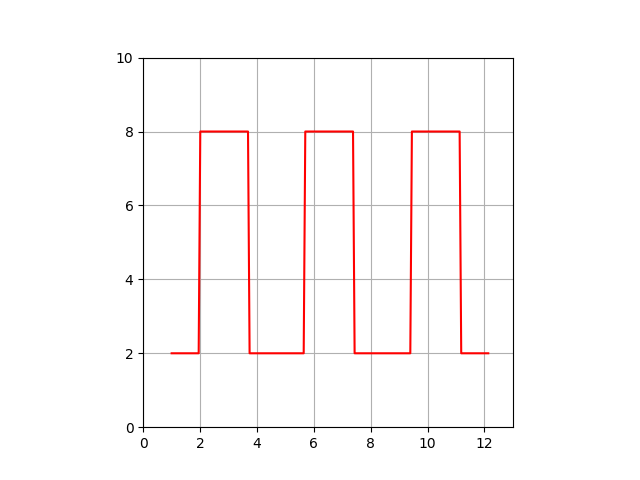
\includegraphics[width=1.0\linewidth]{images/t1_init.png}
    \caption{График квадратной волны}
    \label{fig:placeholder}
\end{figure}

Вычислим коэффициенты ряда Фурье
\[
a_0 = \frac{1}{T}\int_{t_0}^{t_2}f(x)dx = \frac{1}{T}(\int_{t_0}^{t_1}adx + \int_{t_1}^{t_2}bdx) = \frac{1}{T}(a(t_1 - t_0) + b(t_2 - t_1))
\]
\[
a_n = \frac{1}{T}\int_{t_0}^{t_2}f(x)cos(\omega_nx)dx = \frac{1}{T}(\int_{t_0}^{t_1}a\cdot cos(\omega_nx)dx + \int_{t_1}^{t_2}b\cdot cos(\omega_nx)dx) =
\]
\[
= \frac{1}{T\cdot\omega_n}(a(sin(\omega_nt_1) - sin(\omega_nt_0)) +b(sin(\omega_nt_2) - sin(\omega_nt_1)))
\]
\[
b_n = \frac{1}{T}\int_{t_0}^{t_2}f(x)sin(\omega_nx)dx = \frac{1}{T}(\int_{t_0}^{t_1}a\cdot sin(\omega_nx)dx + \int_{t_1}^{t_2}b\cdot sin(\omega_nx)dx) =
\]
\[
= \frac{1}{T\cdot\omega_n}(a(cos(\omega_nt_0) - cos(\omega_nt_1)) +b(cos(\omega_nt_1) - cos(\omega_nt_2)))
\]

Для комплексного ряда Фурье

\[
c_n = \frac{1}{T}\int_{t_0}^{t_1}f(x)e^{-i\omega_nx}dx = \frac{1}{T}(\int_{t_0}^{t_1}ae^{-i\omega_nx}dx + \int_{t_1}^{t_2}be^{-i\omega_nx}dx) =
\]
\[
=\frac{1}{-iT\omega_n}(a(e^{-i\omega_nt_1} - e^{-i\omega_nt_0}) + b(e^{-i\omega_nt_2} - e^{-i\omega_nt_1}))
\]
Но для \(n=0\) общая формула не подходит(в знаменателе - ноль), рассмотрим этот случай отдельно
\[
c_0 = \frac{1}{T}\int_{t_0}^{t_1}f(x)e^{-ix\cdot0}dx = \frac{1}{T}\int_{t_0}^{t_1}f(x)dx = \frac{1}{T}(a(t_1 - t_0) + b(t_2 - t_1))
\]

Все эти коэффициенты неочевидны. Программно(см. Приложение) вычислим коэффициенты для \(N=2\)(коэффициенты приведены с точностью до тысячных):
\[
a_0 = 6.426
\]
\[
a_1 = 2.274
\]
\[
a_2 = -0.601
\]

\[
b_1 = -1.640
\]
\[
b_2 = 1.807
\]

\[
c_0 = 6.426
\]
\[
c_{\pm 1} = 1.137 \pm i0.820
\]
\[
c_{\pm 2} = -0.300 \pm i0.903
\]

\begin{figure}[H]
    \centering
    
    
    \begin{subfigure}[b]{0.48\textwidth}
        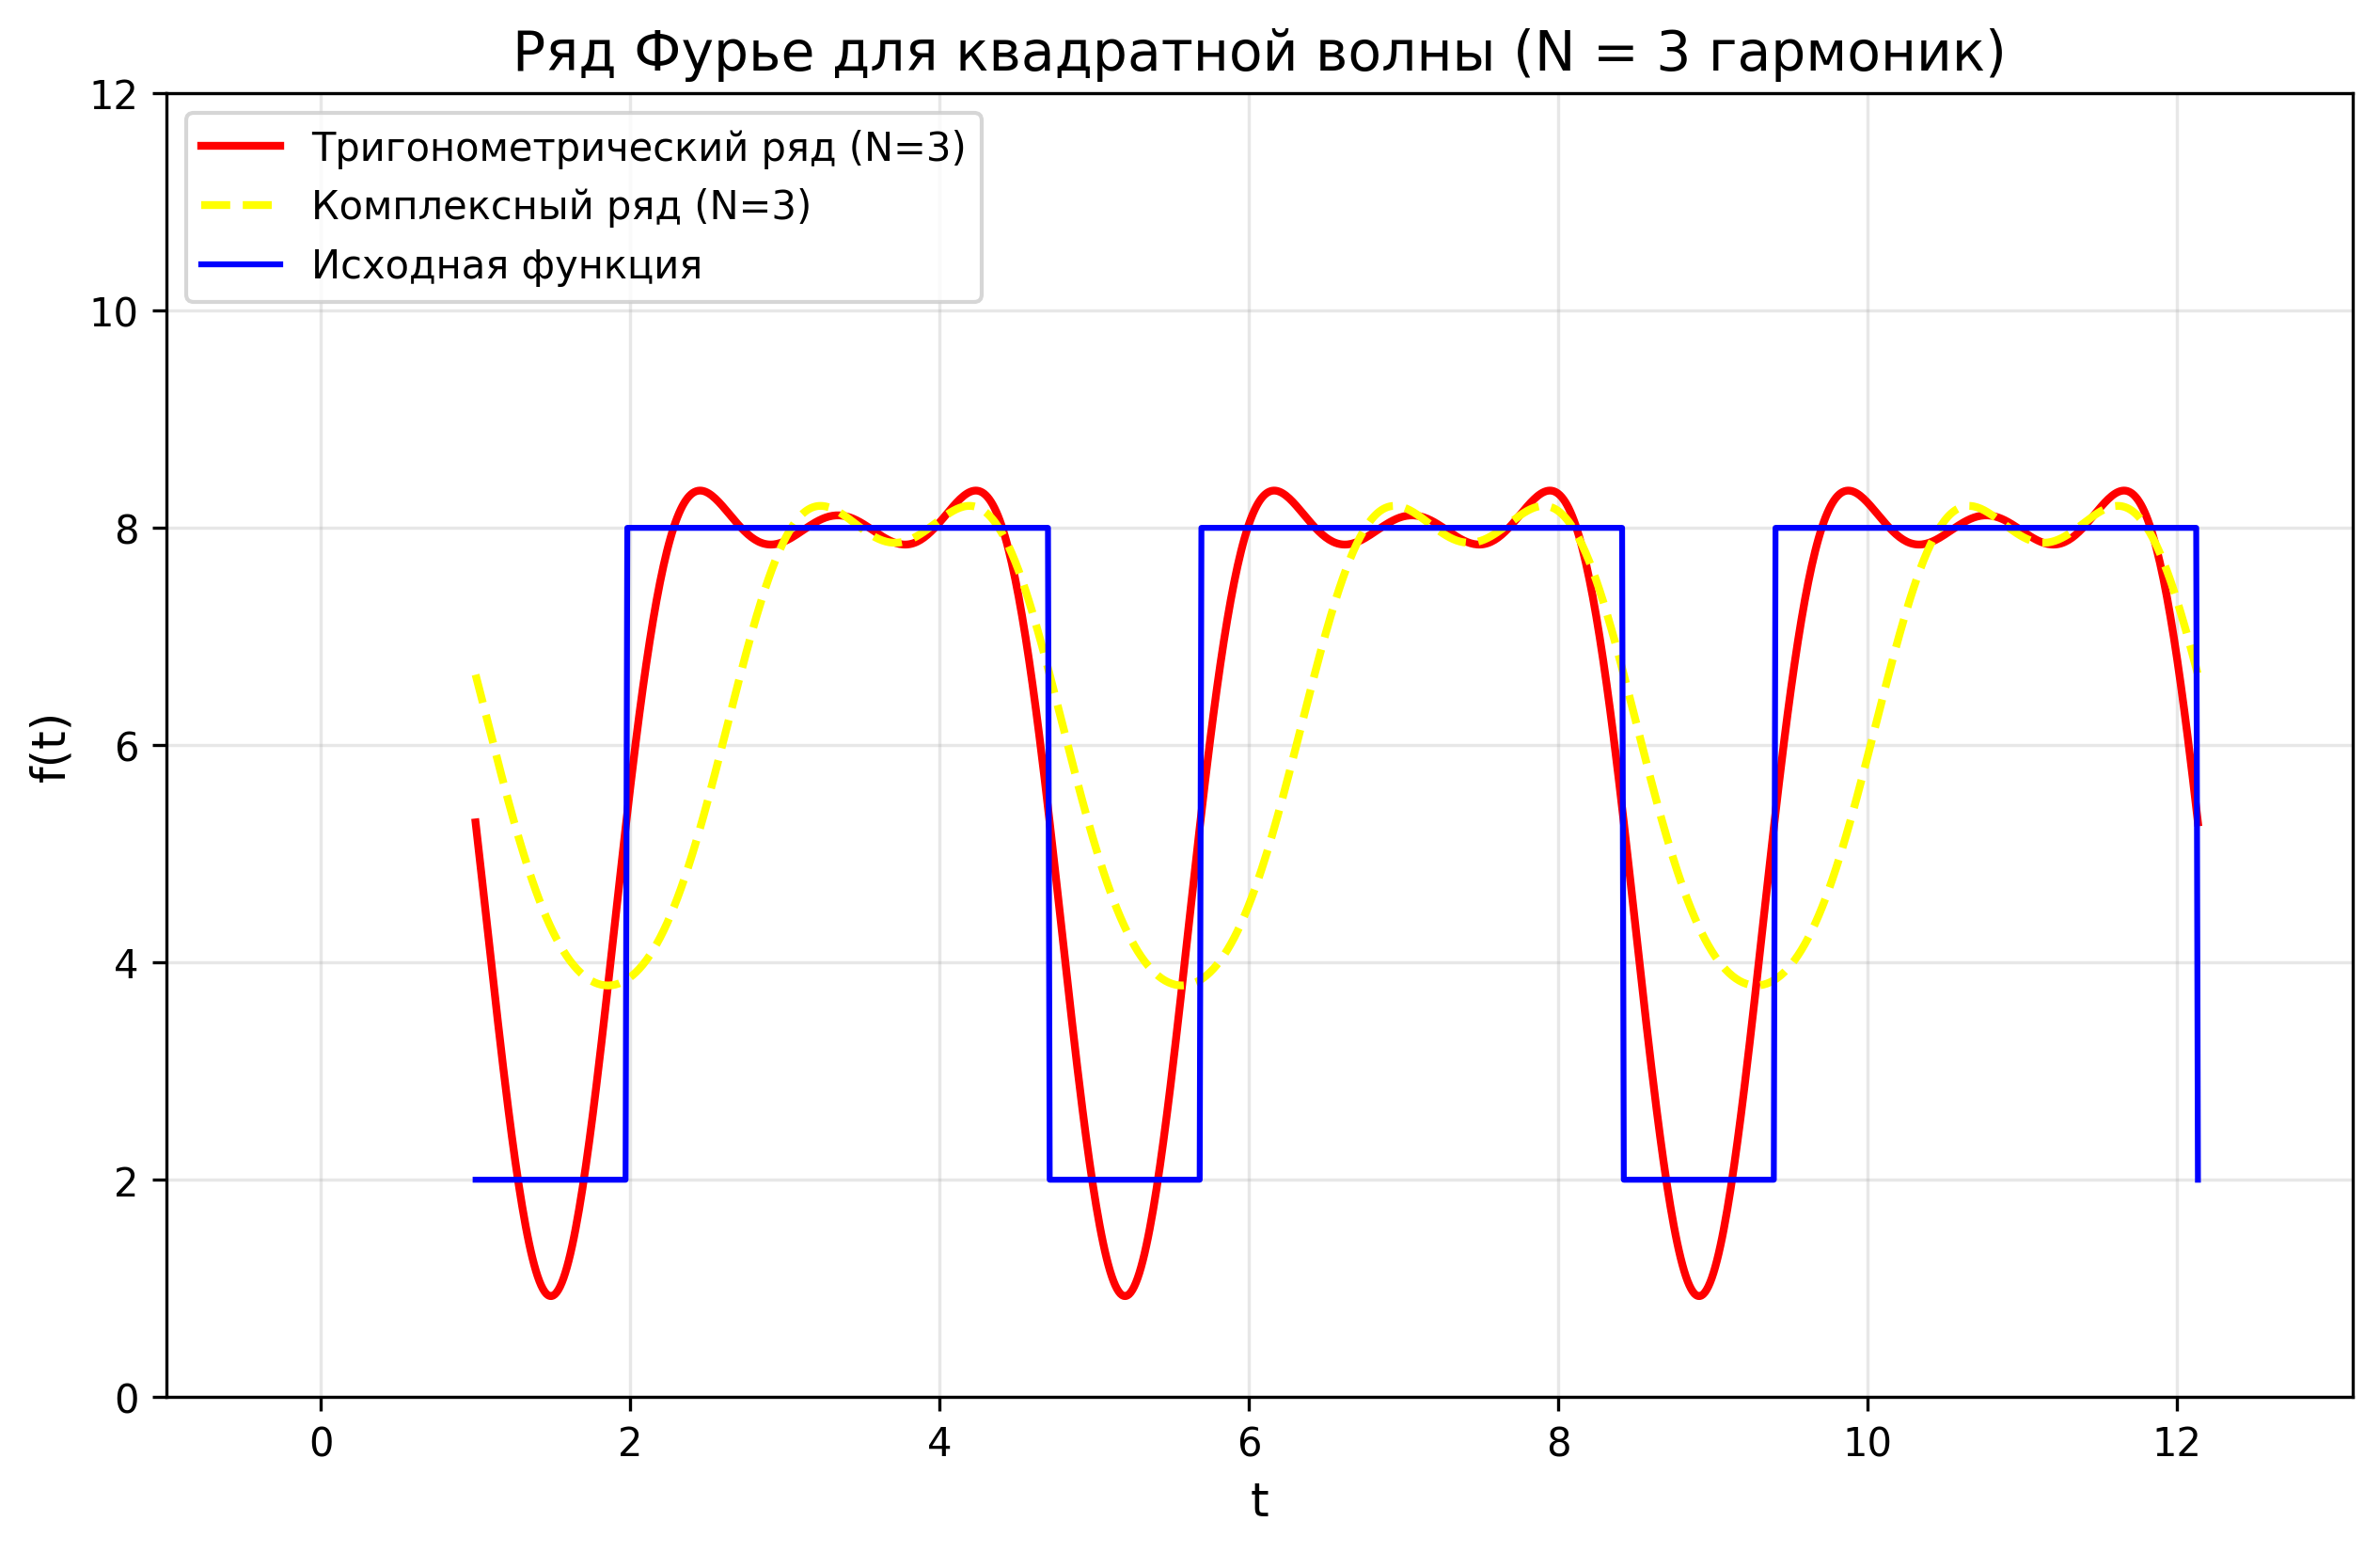
\includegraphics[width=\textwidth]{images/t1_3.png}
        \caption{N = 3 гармоники}
        \label{fig:n3}
    \end{subfigure}
    \hfill
    \begin{subfigure}[b]{0.48\textwidth}
        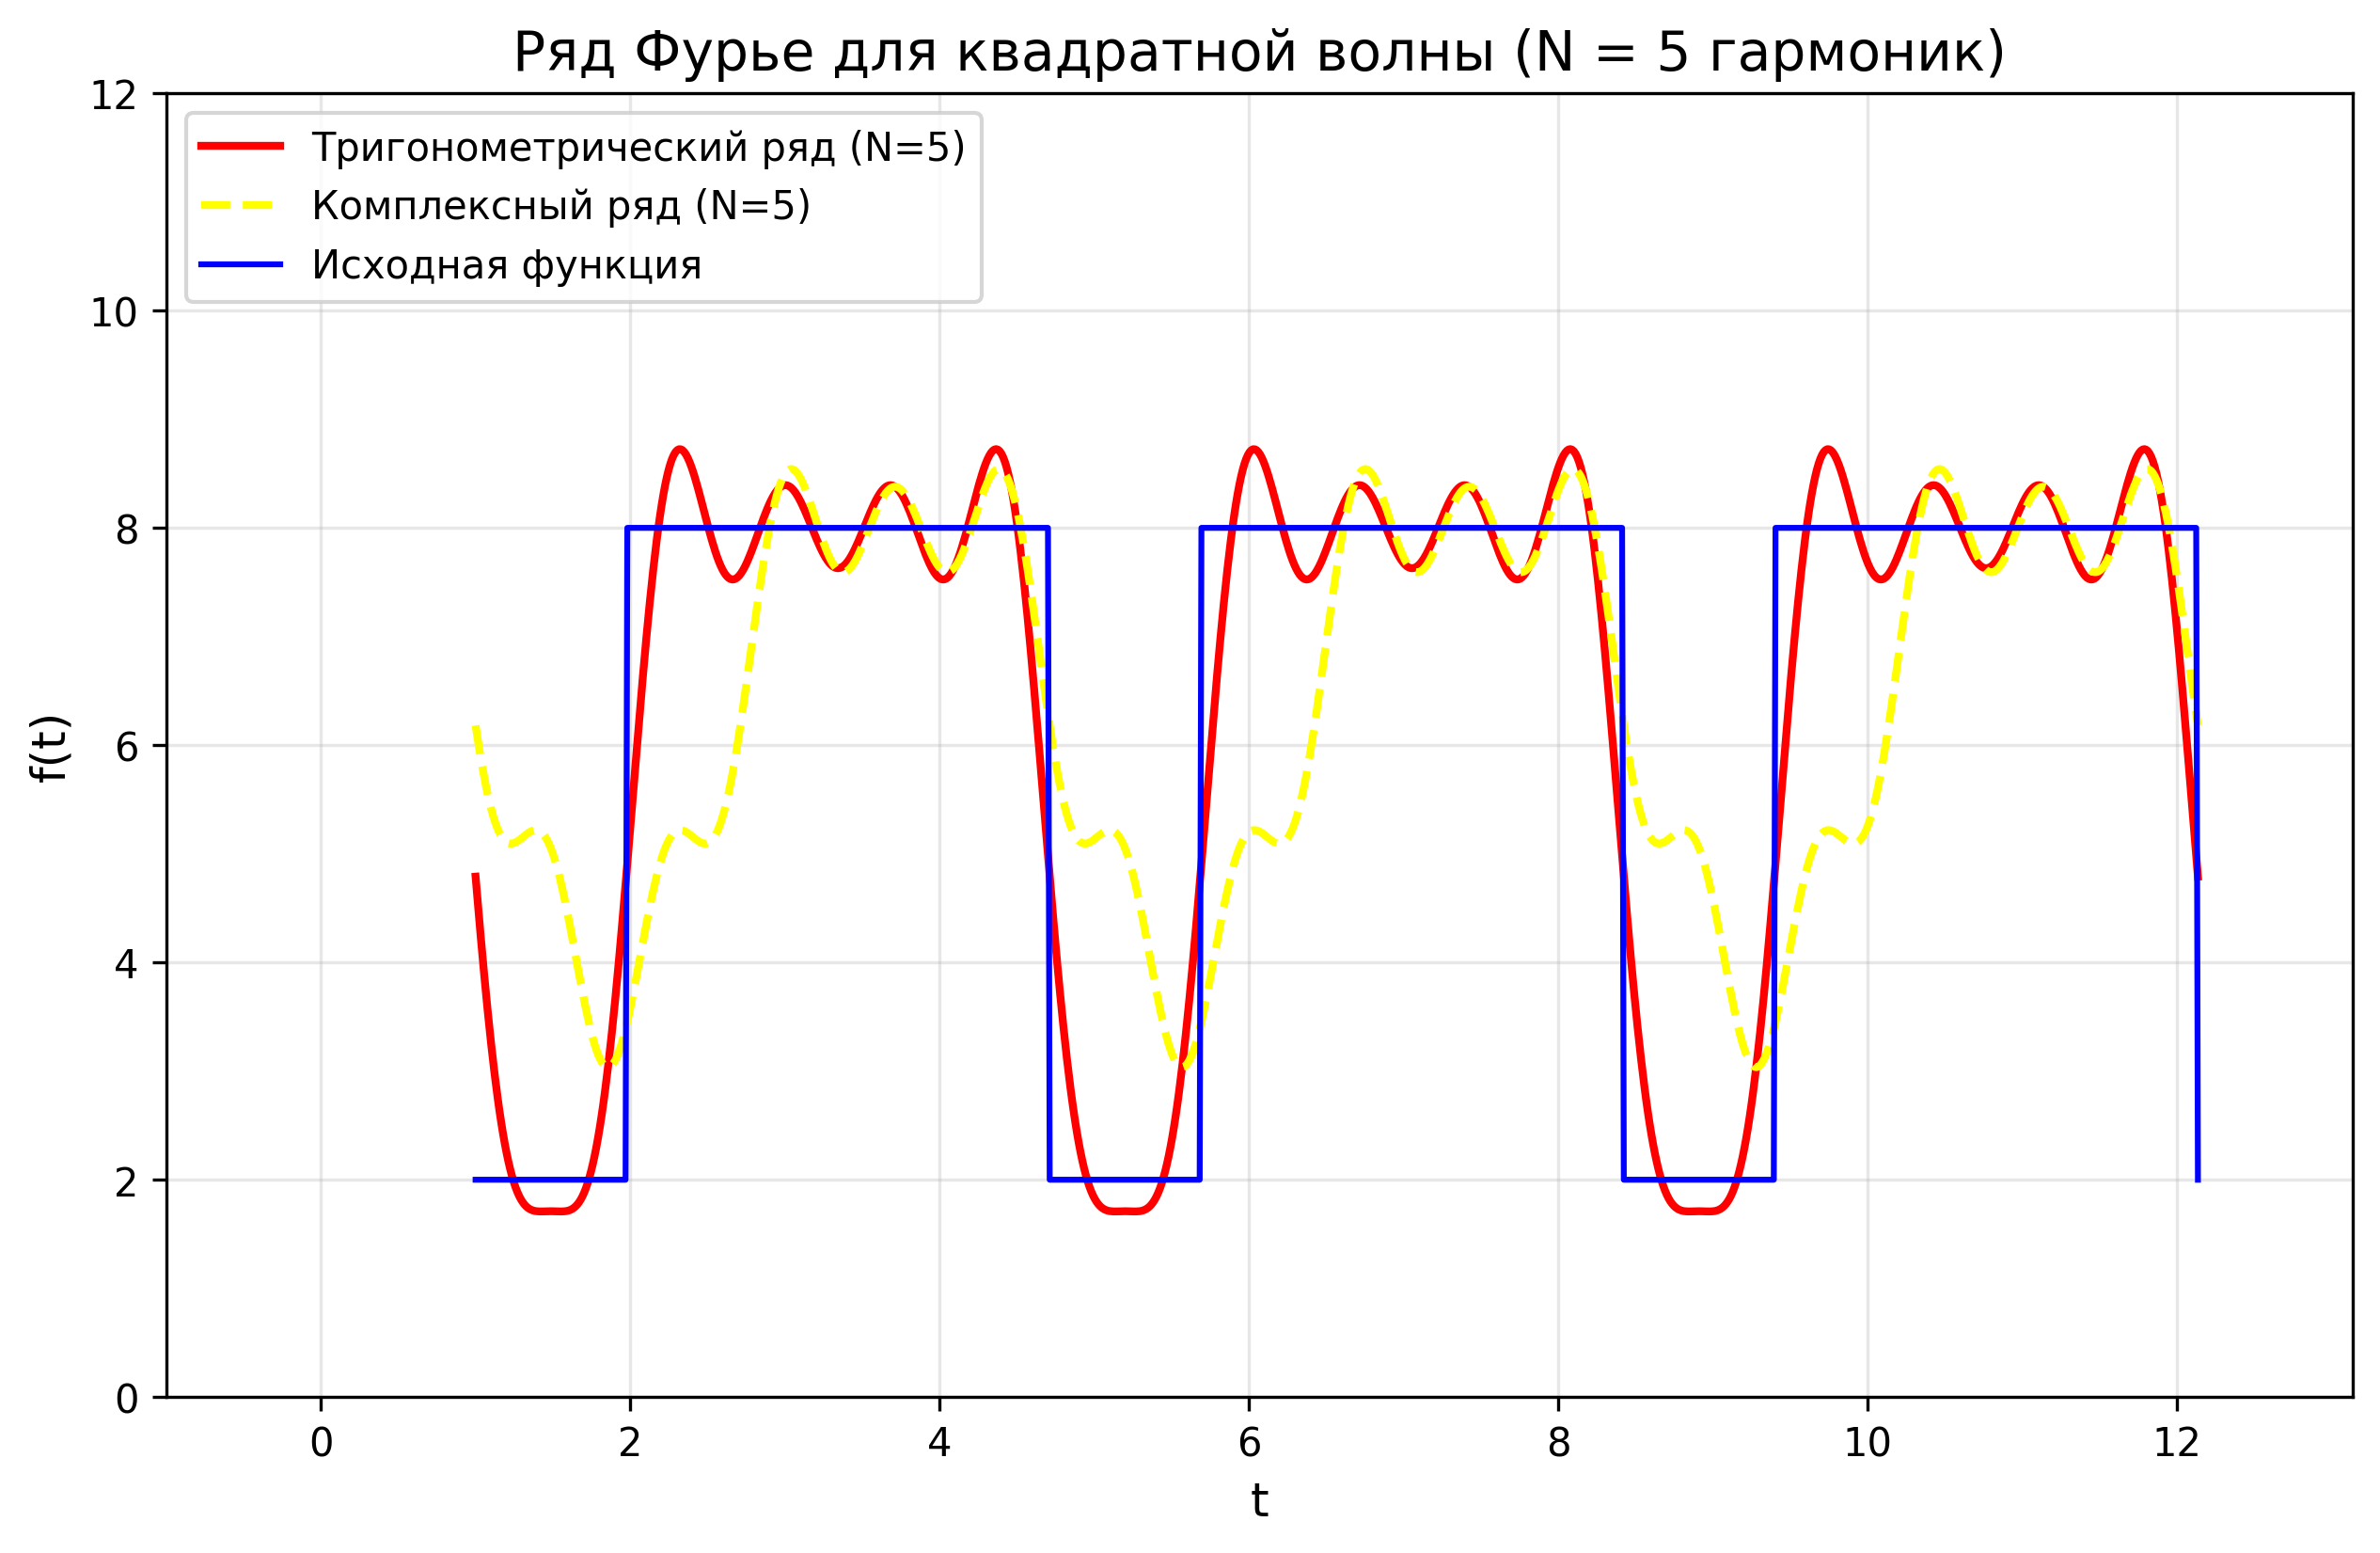
\includegraphics[width=\textwidth]{images/t1_5.png}
        \caption{N = 5 гармоник}
        \label{fig:n5}
    \end{subfigure}
    
    \vspace{0.5cm}
    
    \begin{subfigure}[b]{0.48\textwidth}
        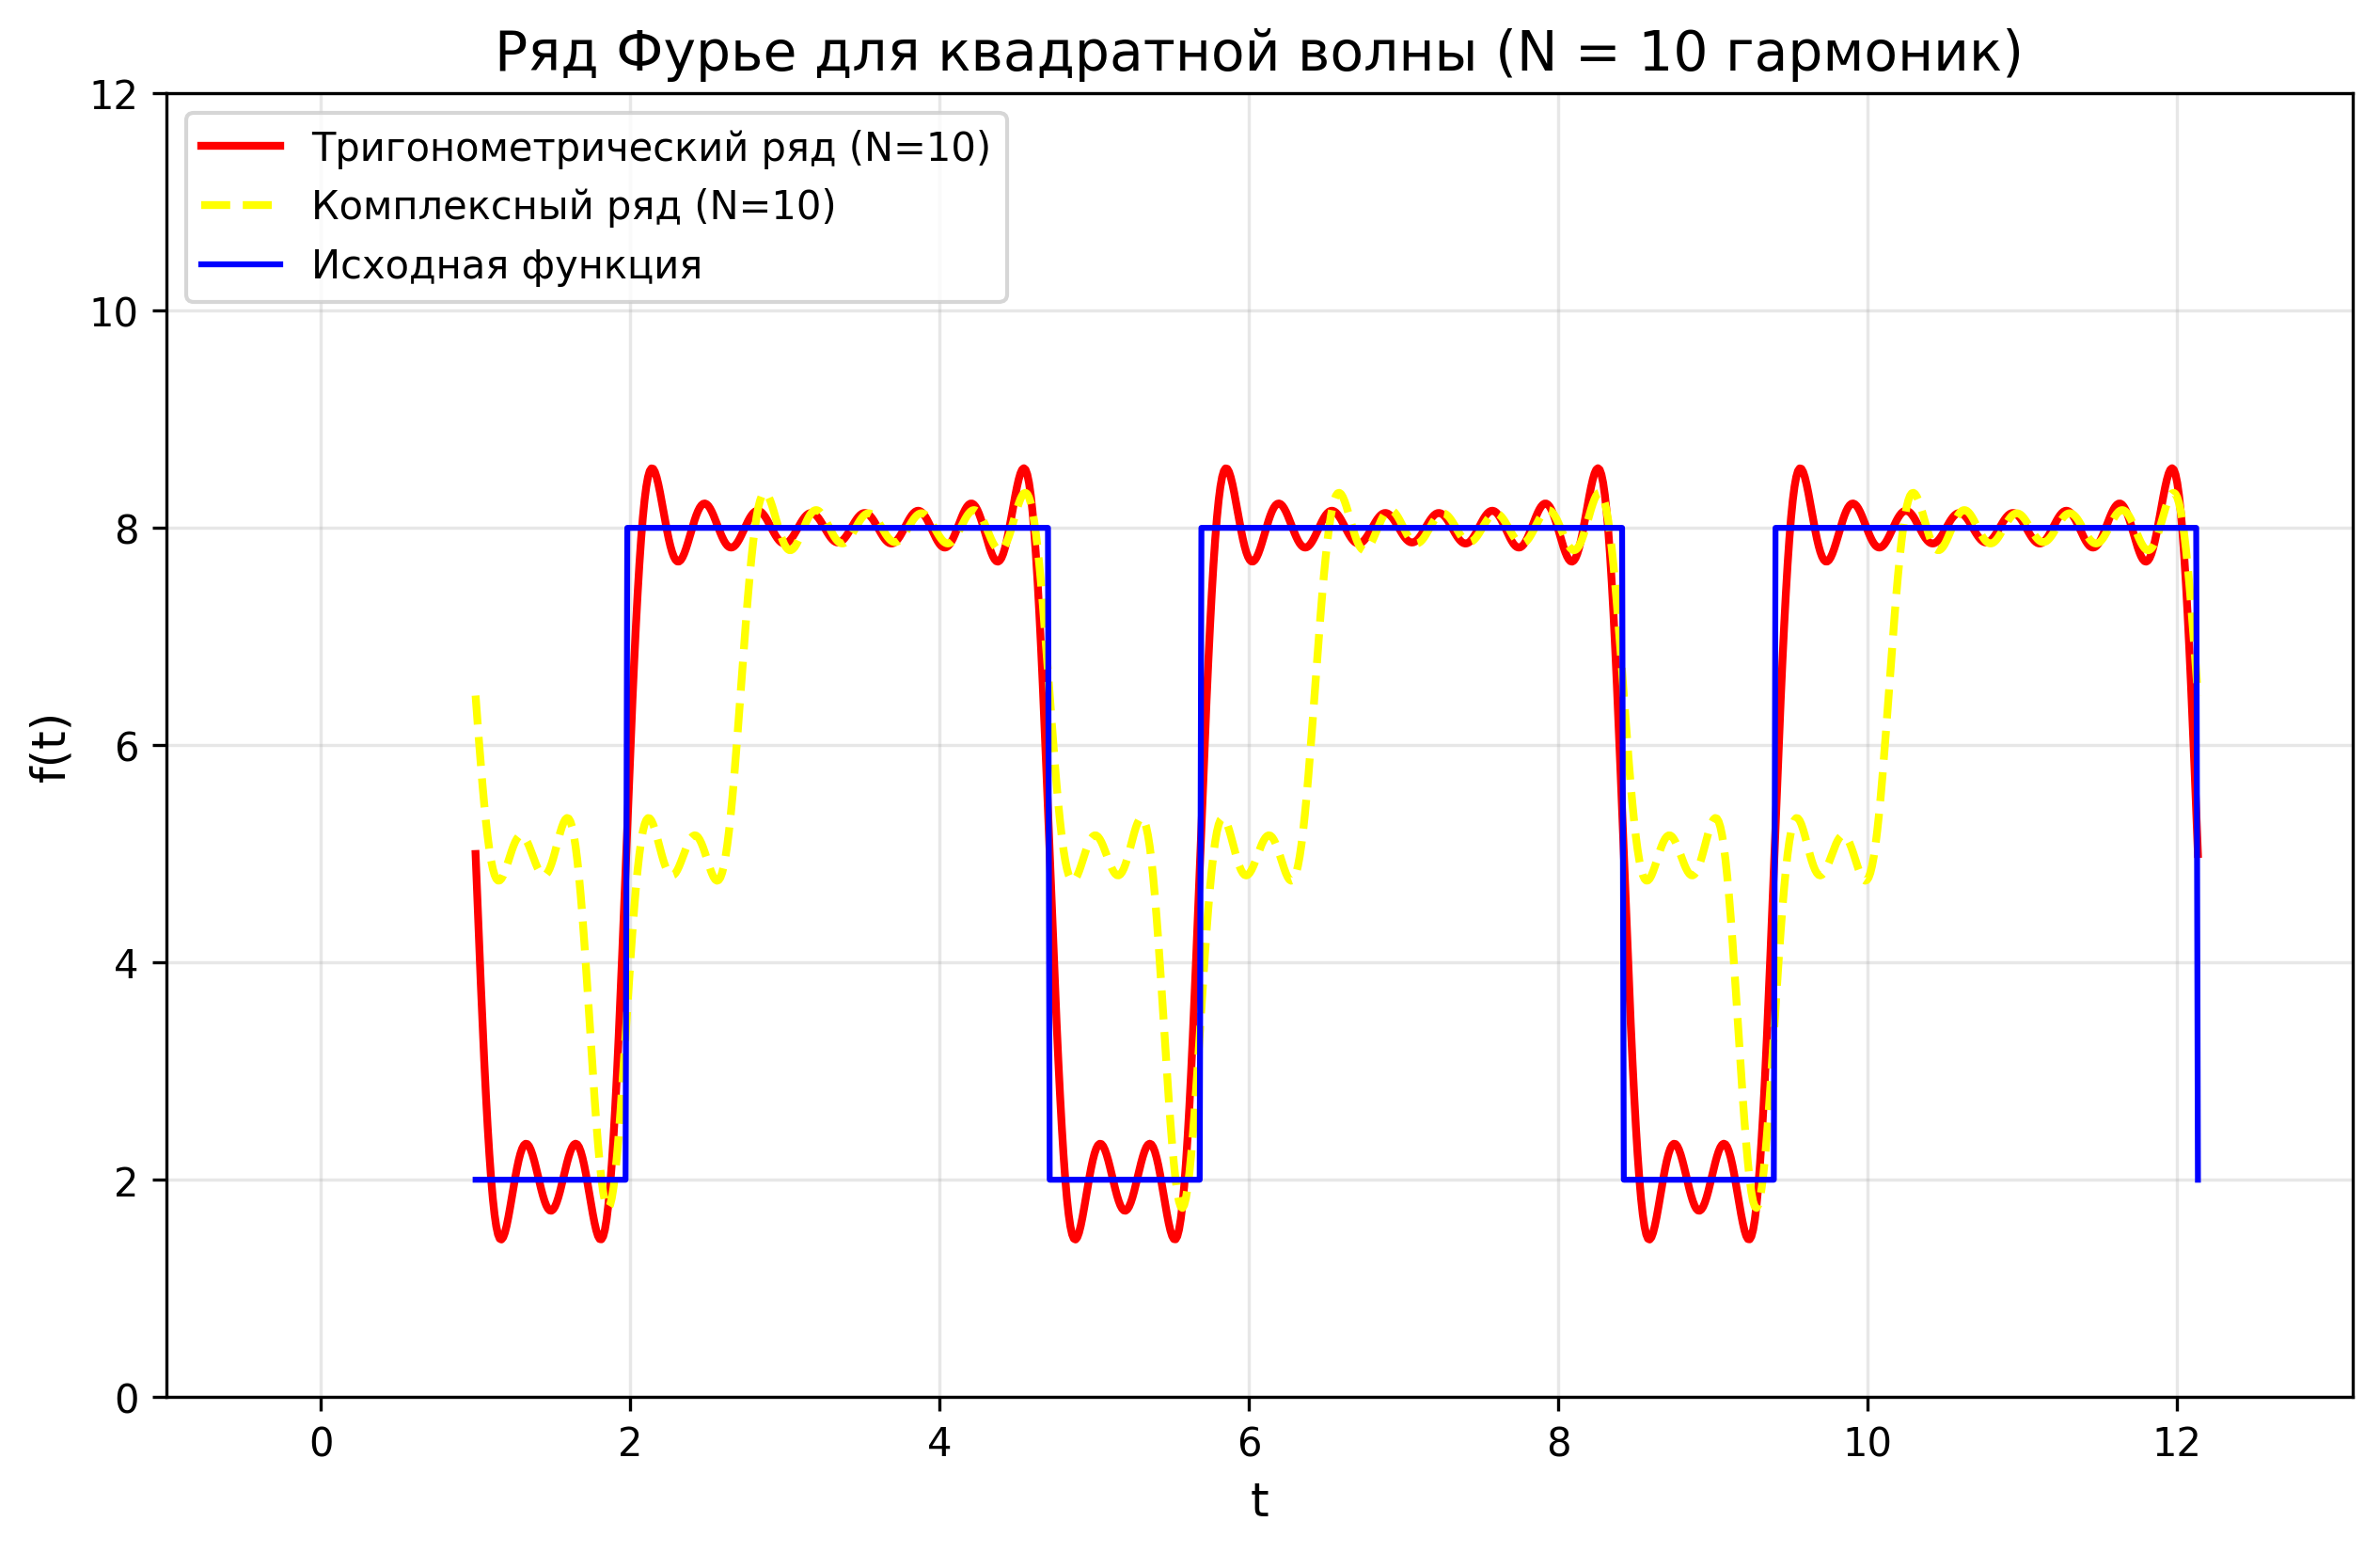
\includegraphics[width=\textwidth]{images/t1_10.png}
        \caption{N = 10 гармоник}
        \label{fig:n10}
    \end{subfigure}
    \hfill
    \begin{subfigure}[b]{0.48\textwidth}
        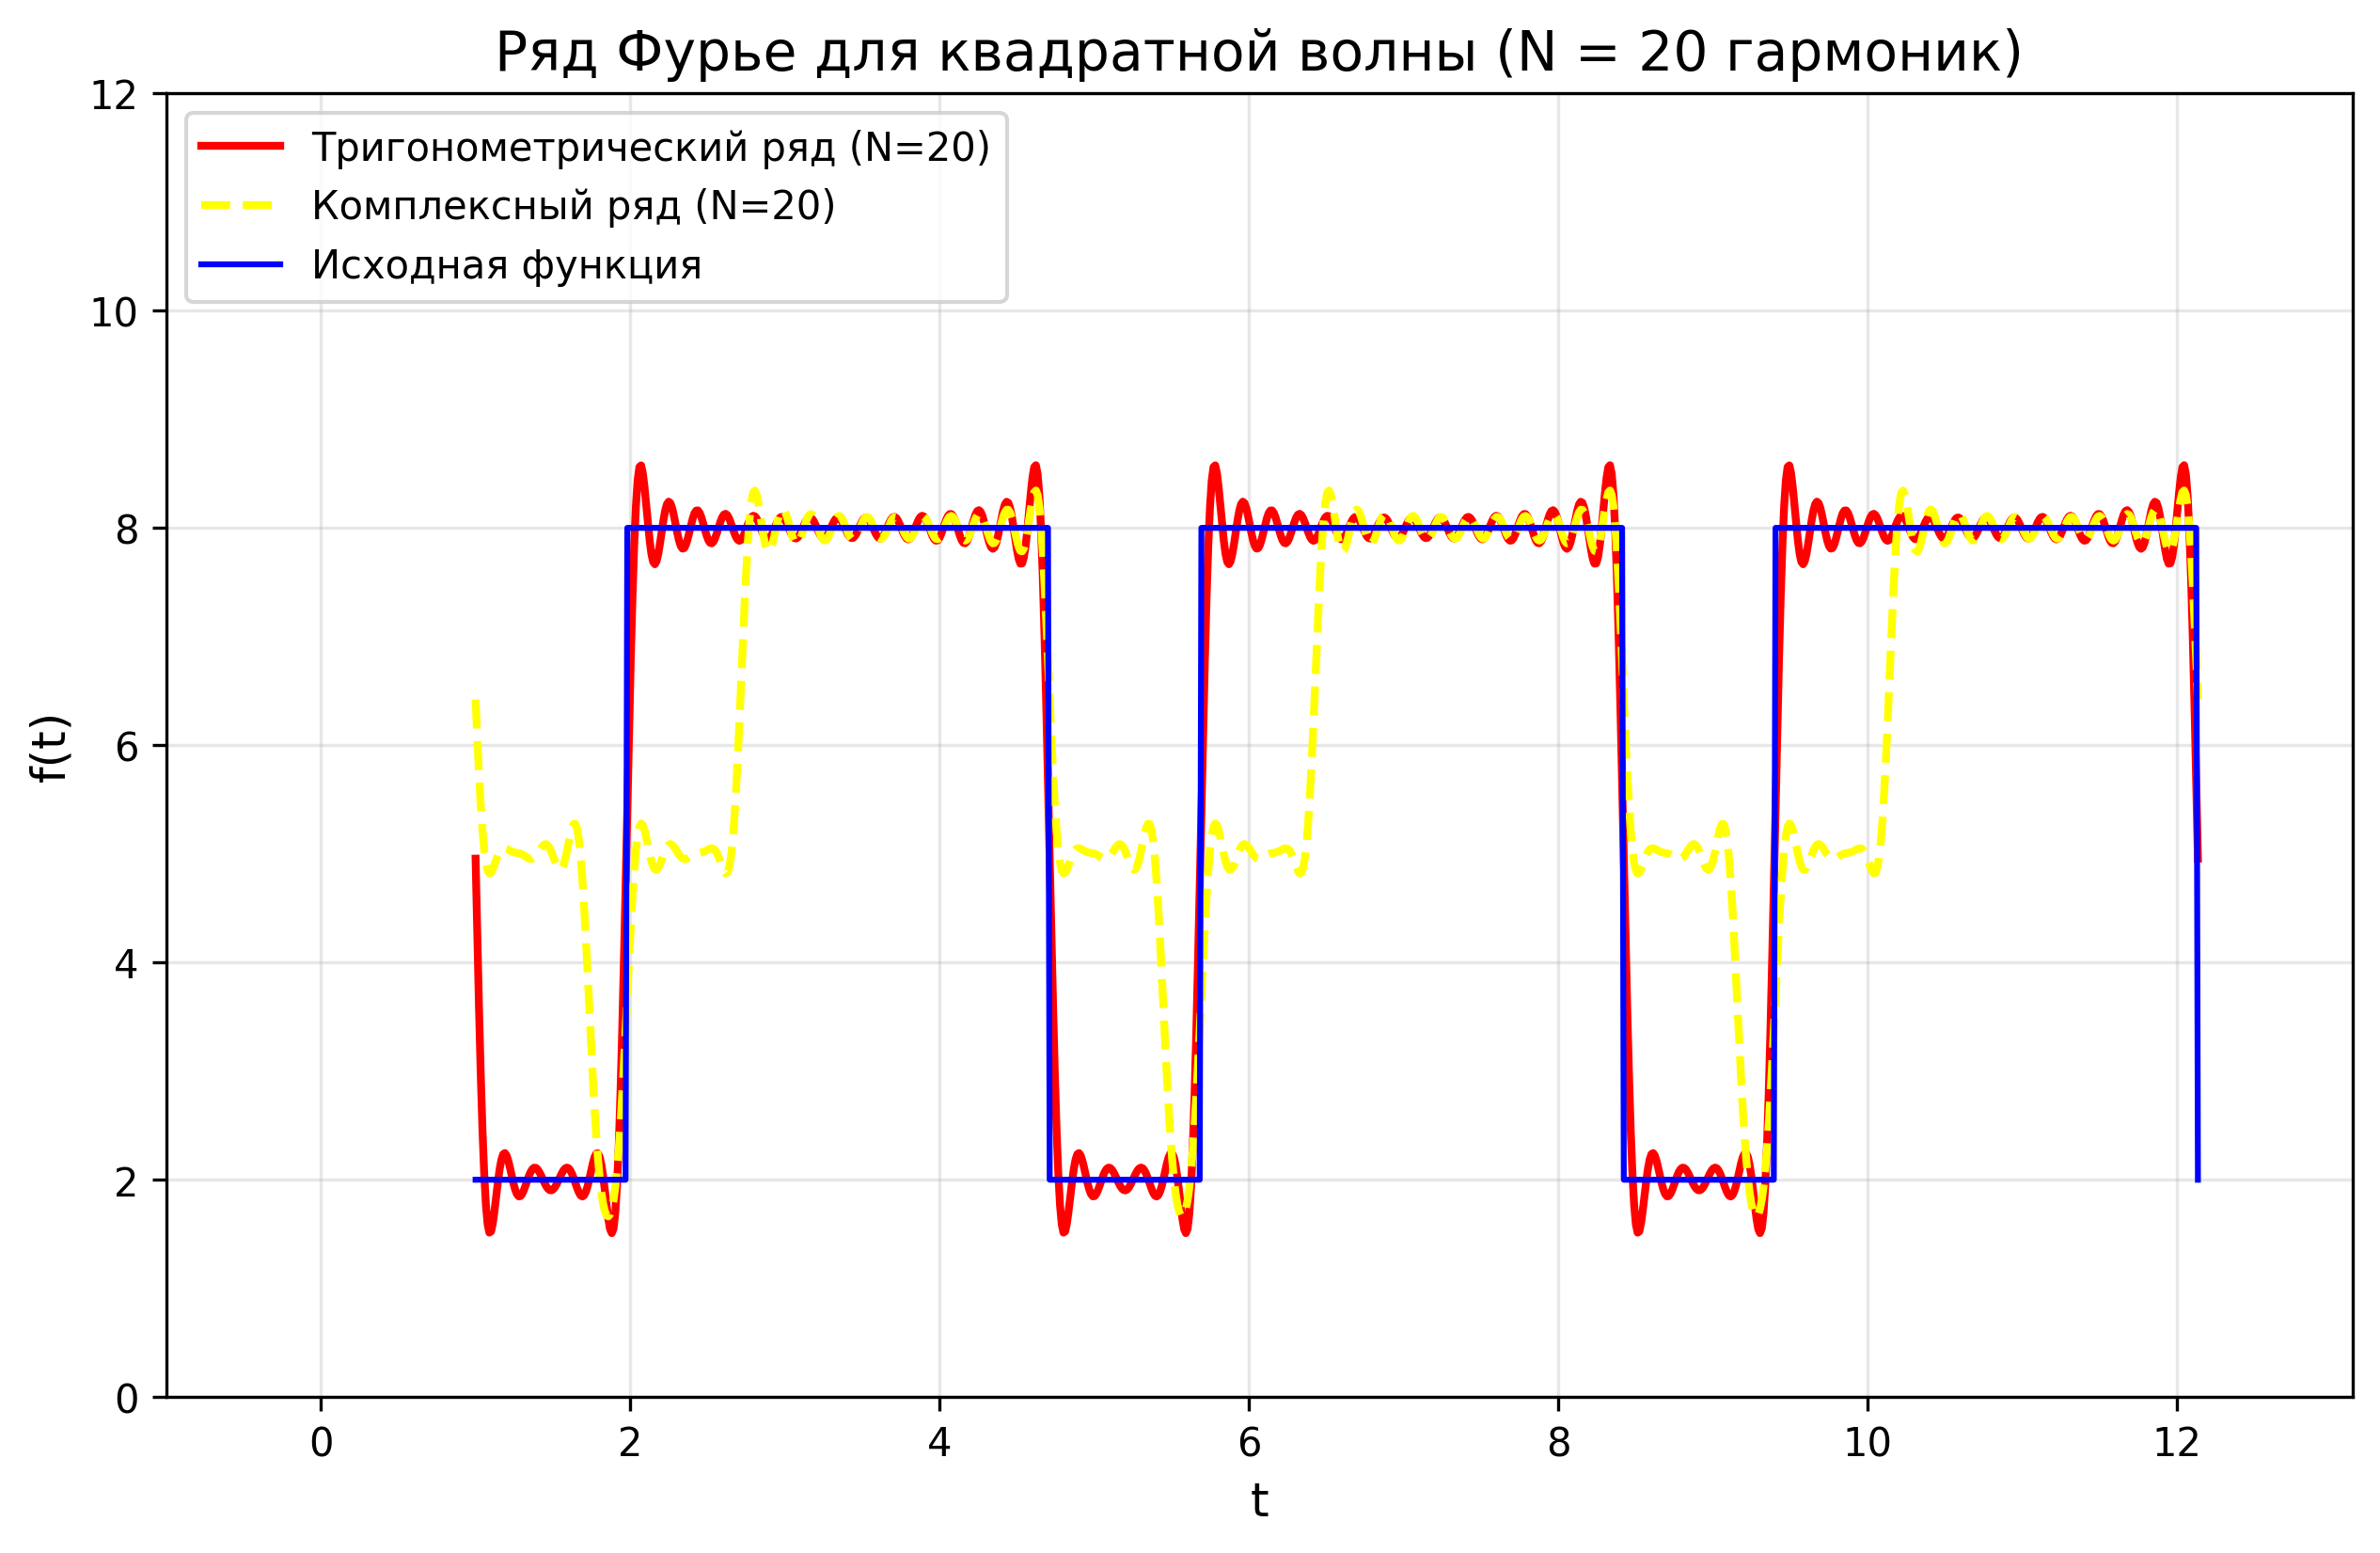
\includegraphics[width=\textwidth]{images/t1_20.png}
        \caption{N = 20 гармоник}
        \label{fig:n20}
    \end{subfigure}
    \vspace{0.5cm}
    \begin{subfigure}[b]{0.48\textwidth}
        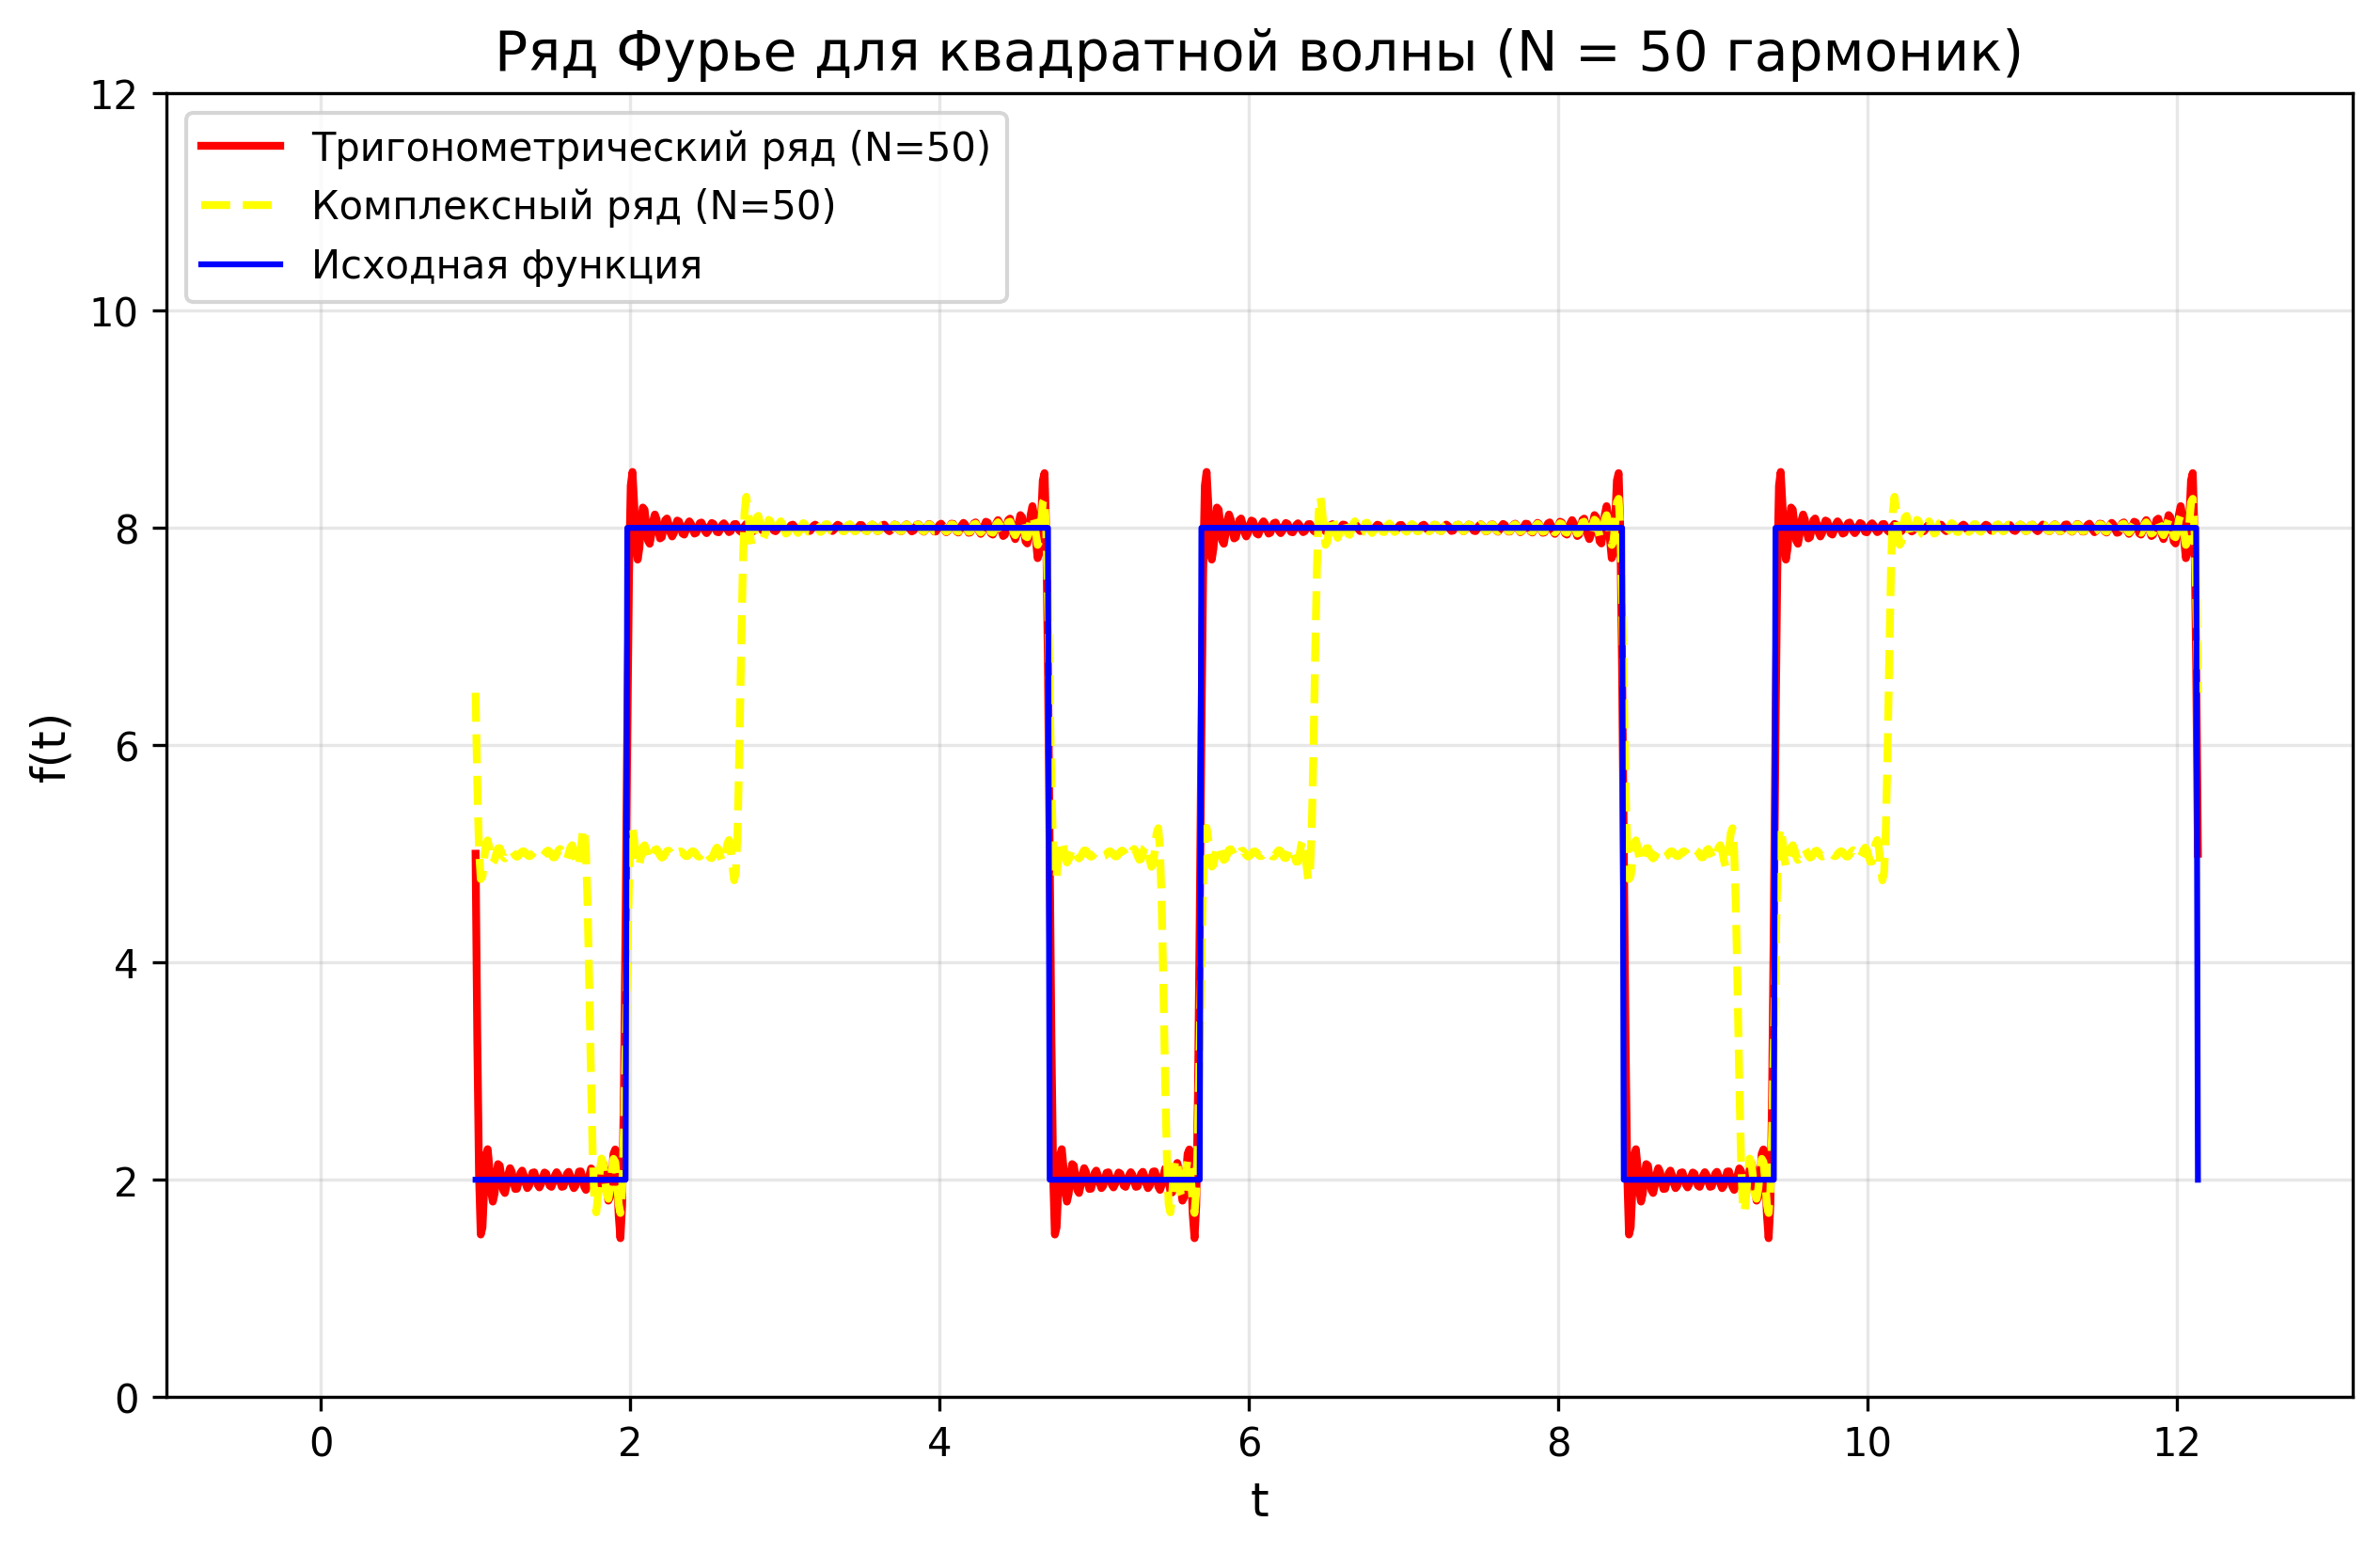
\includegraphics[width=\textwidth]{images/t1_50.png}
        \caption{N = 50 гармоник}
        \label{fig:n50}
    \end{subfigure}
        
    \caption{Приближение квадратной волны рядом Фурье для разного количества гармоник}
    \label{fig:fourier_grid}
\end{figure}





\subsection{Чётная переодическая функция}
Возьмём чётную переодическую функцию
\[
f(x) = |sin(x)|\cdot e^{cos(x)^3}
\]
Её график
\begin{figure}[H]
    \centering
    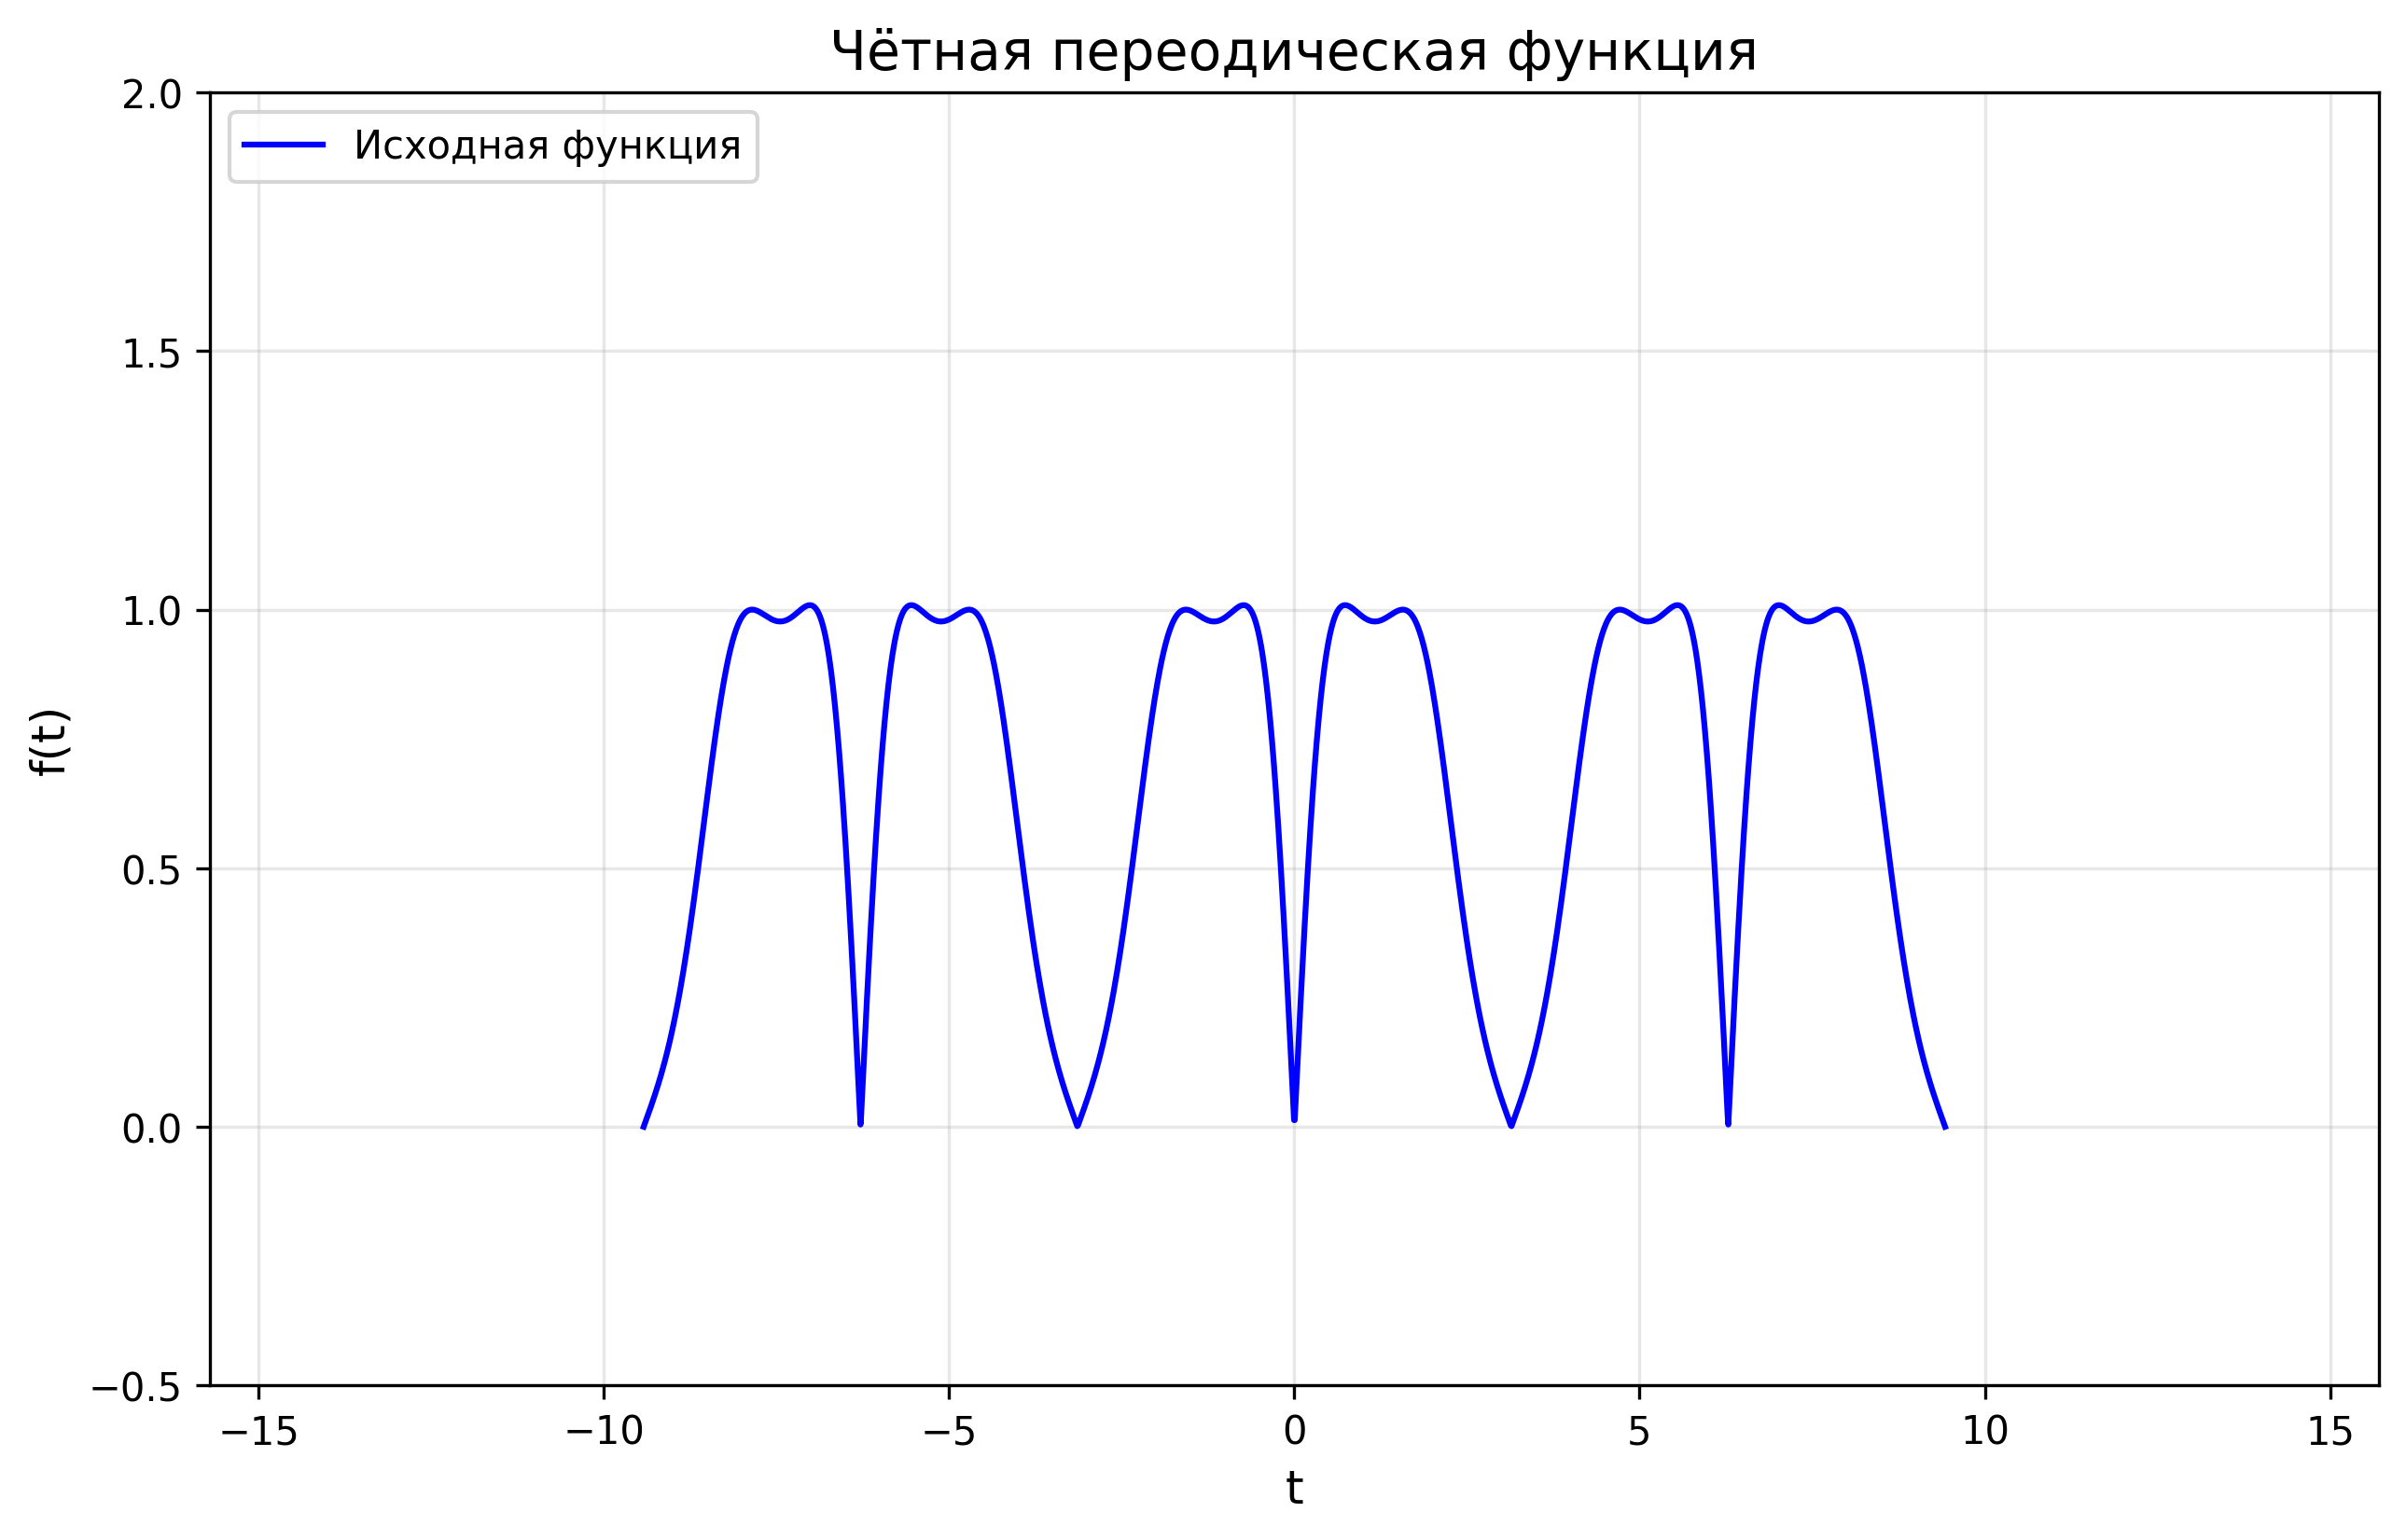
\includegraphics[width=1.0\linewidth]{images/t2_0.png}
    \caption{График чётной переодической функции}
    \label{fig:placeholder}
\end{figure}

Аналитическое вычисление интегралов от этой функции(а тем более от произвдедения её на sin и cos) если и возможно, то очень затруднительно. Поэтому все коэффициенты вычисляются численно, при помощи кода.

Коэффициенты b, очевидно нулевые, так как это нечтная функция. Остальные коэффициенты неочевидны
\[
a_0 = 0.684
\]
\[
a_1 = 0.275
\]
\[
a_2 = -0.371
\]

\[
b_1 = b_2 = 0
\]

\[
c_0 = 0.684
\]
\[
c_{\pm 1} = 0.137 \pm 0\cdot i
\]
\[
c_{\pm 2} = -0.185 \pm 0 \cdot i
\]

\begin{figure}[H]
    \centering
    
    
    \begin{subfigure}[b]{0.48\textwidth}
        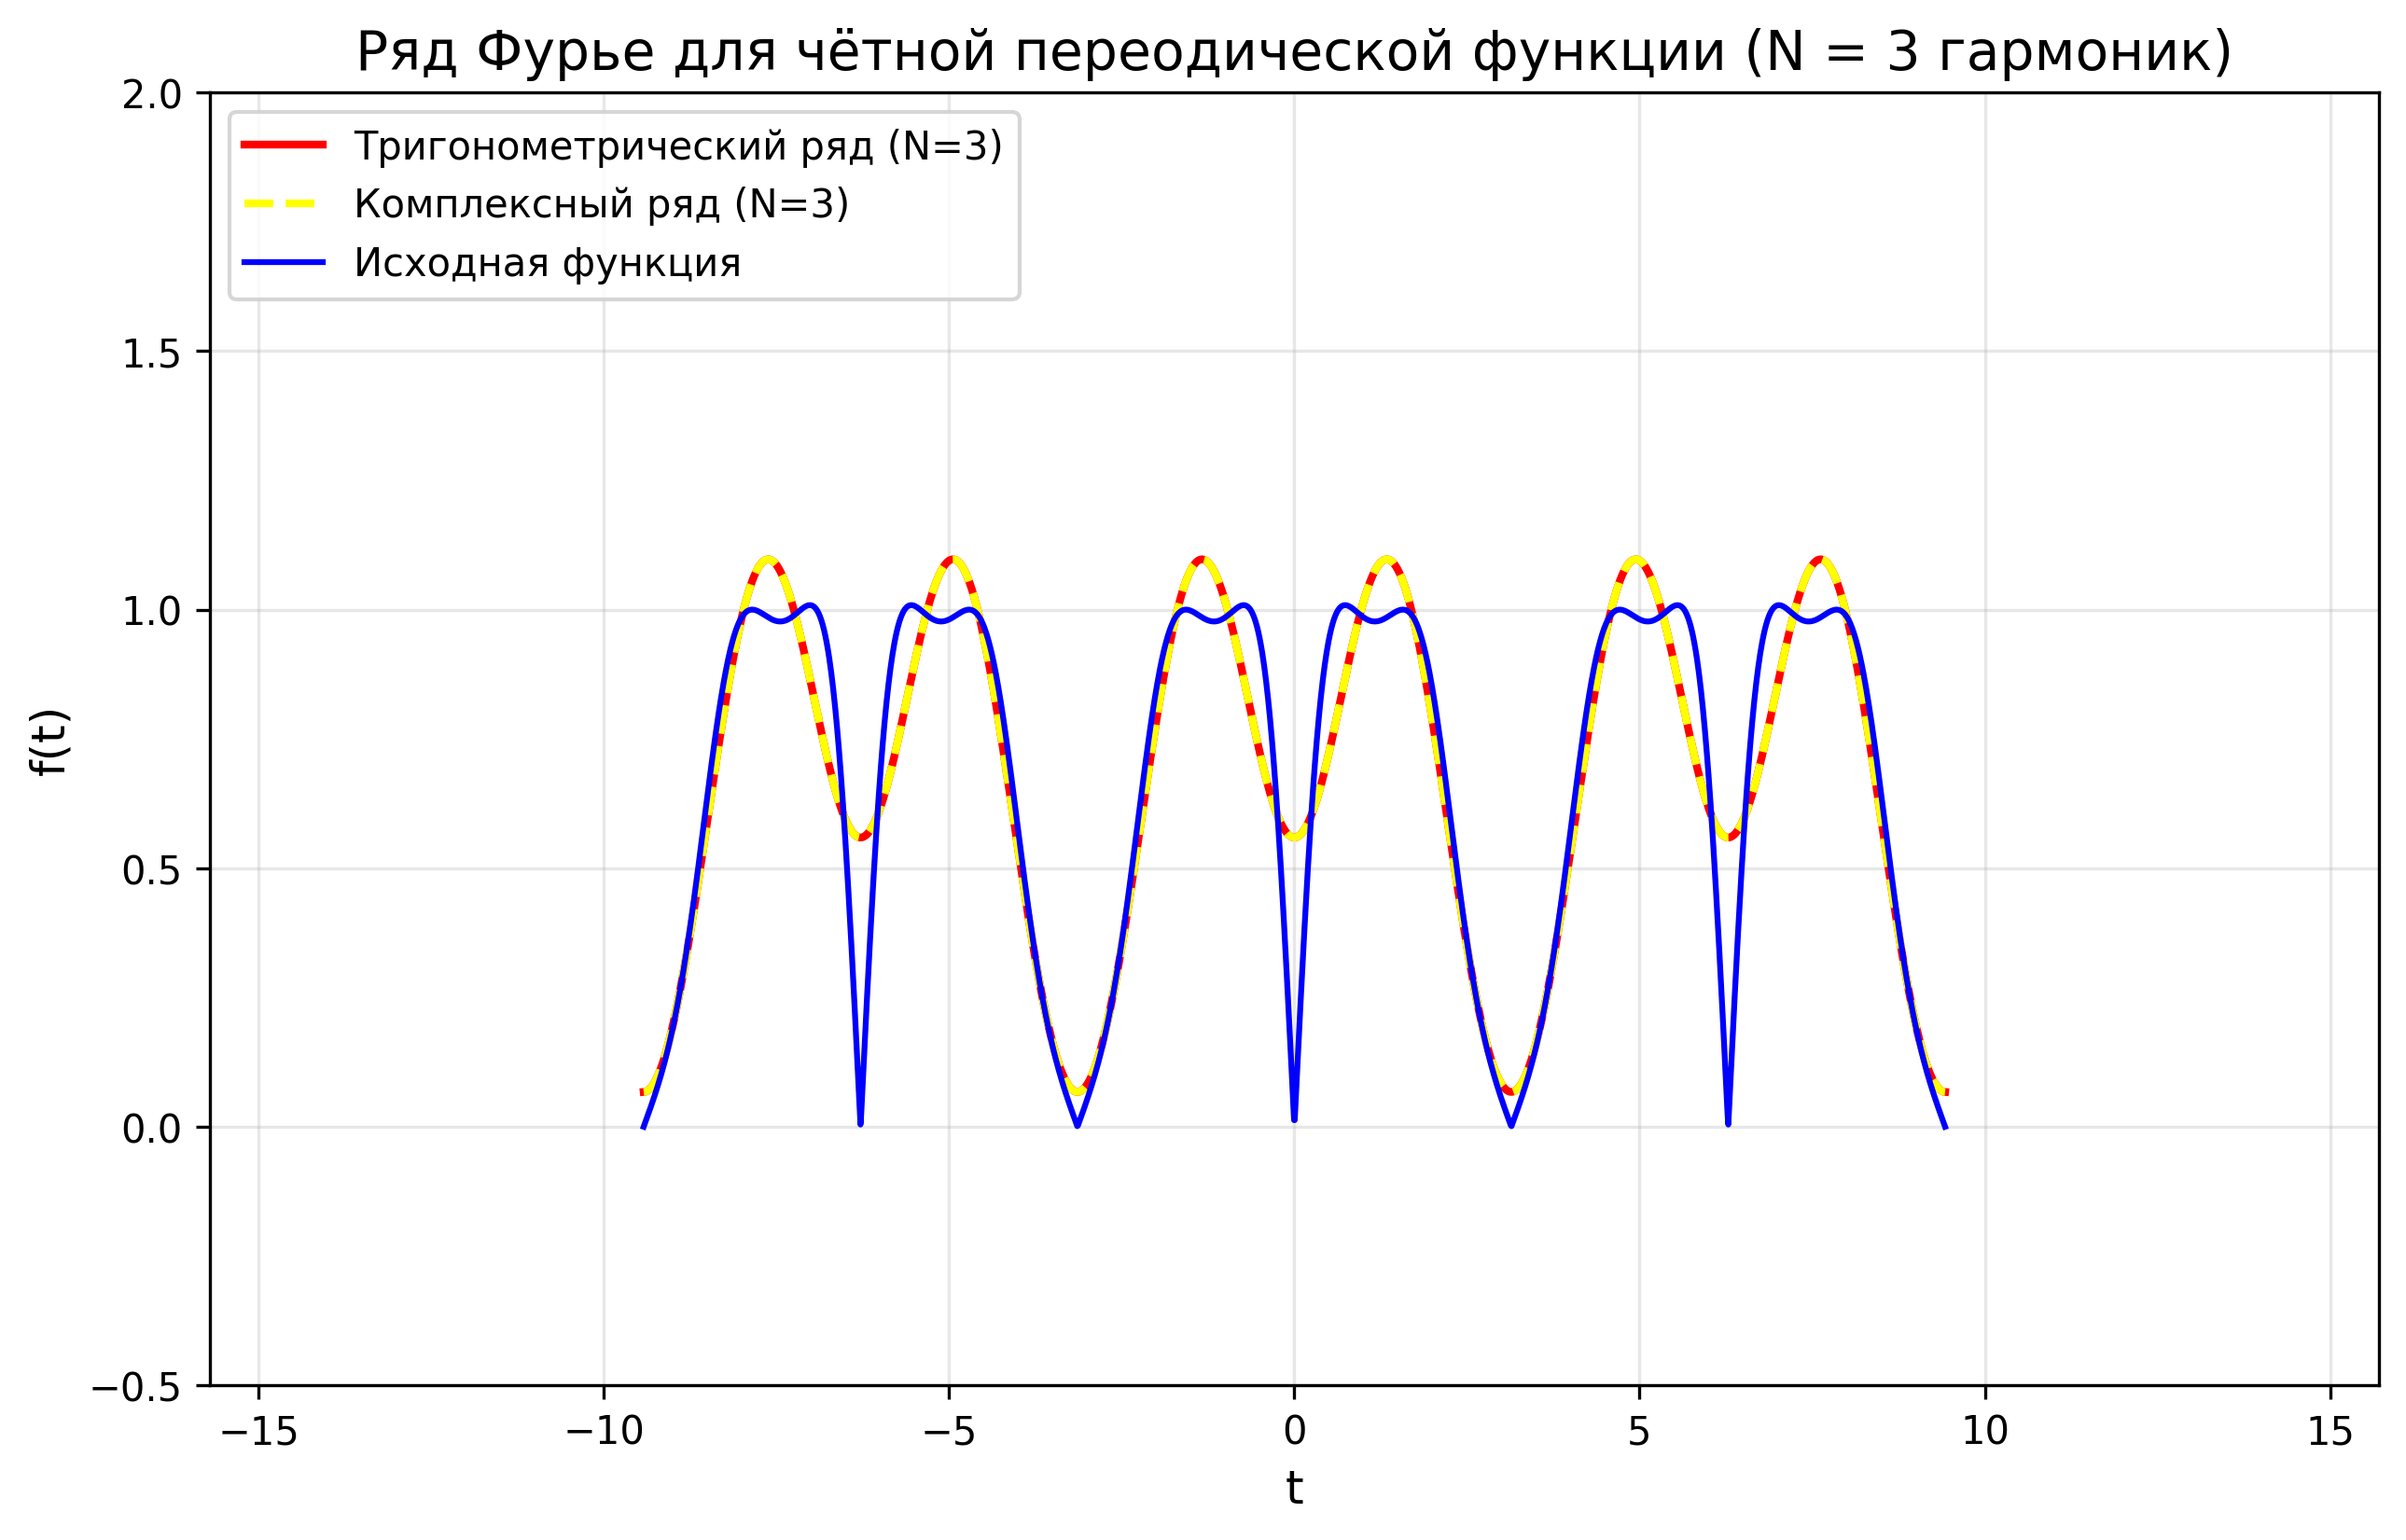
\includegraphics[width=\textwidth]{images/t2_3.png}
        \caption{N = 3 гармоники}
        \label{fig:n3}
    \end{subfigure}
    \hfill
    \begin{subfigure}[b]{0.48\textwidth}
        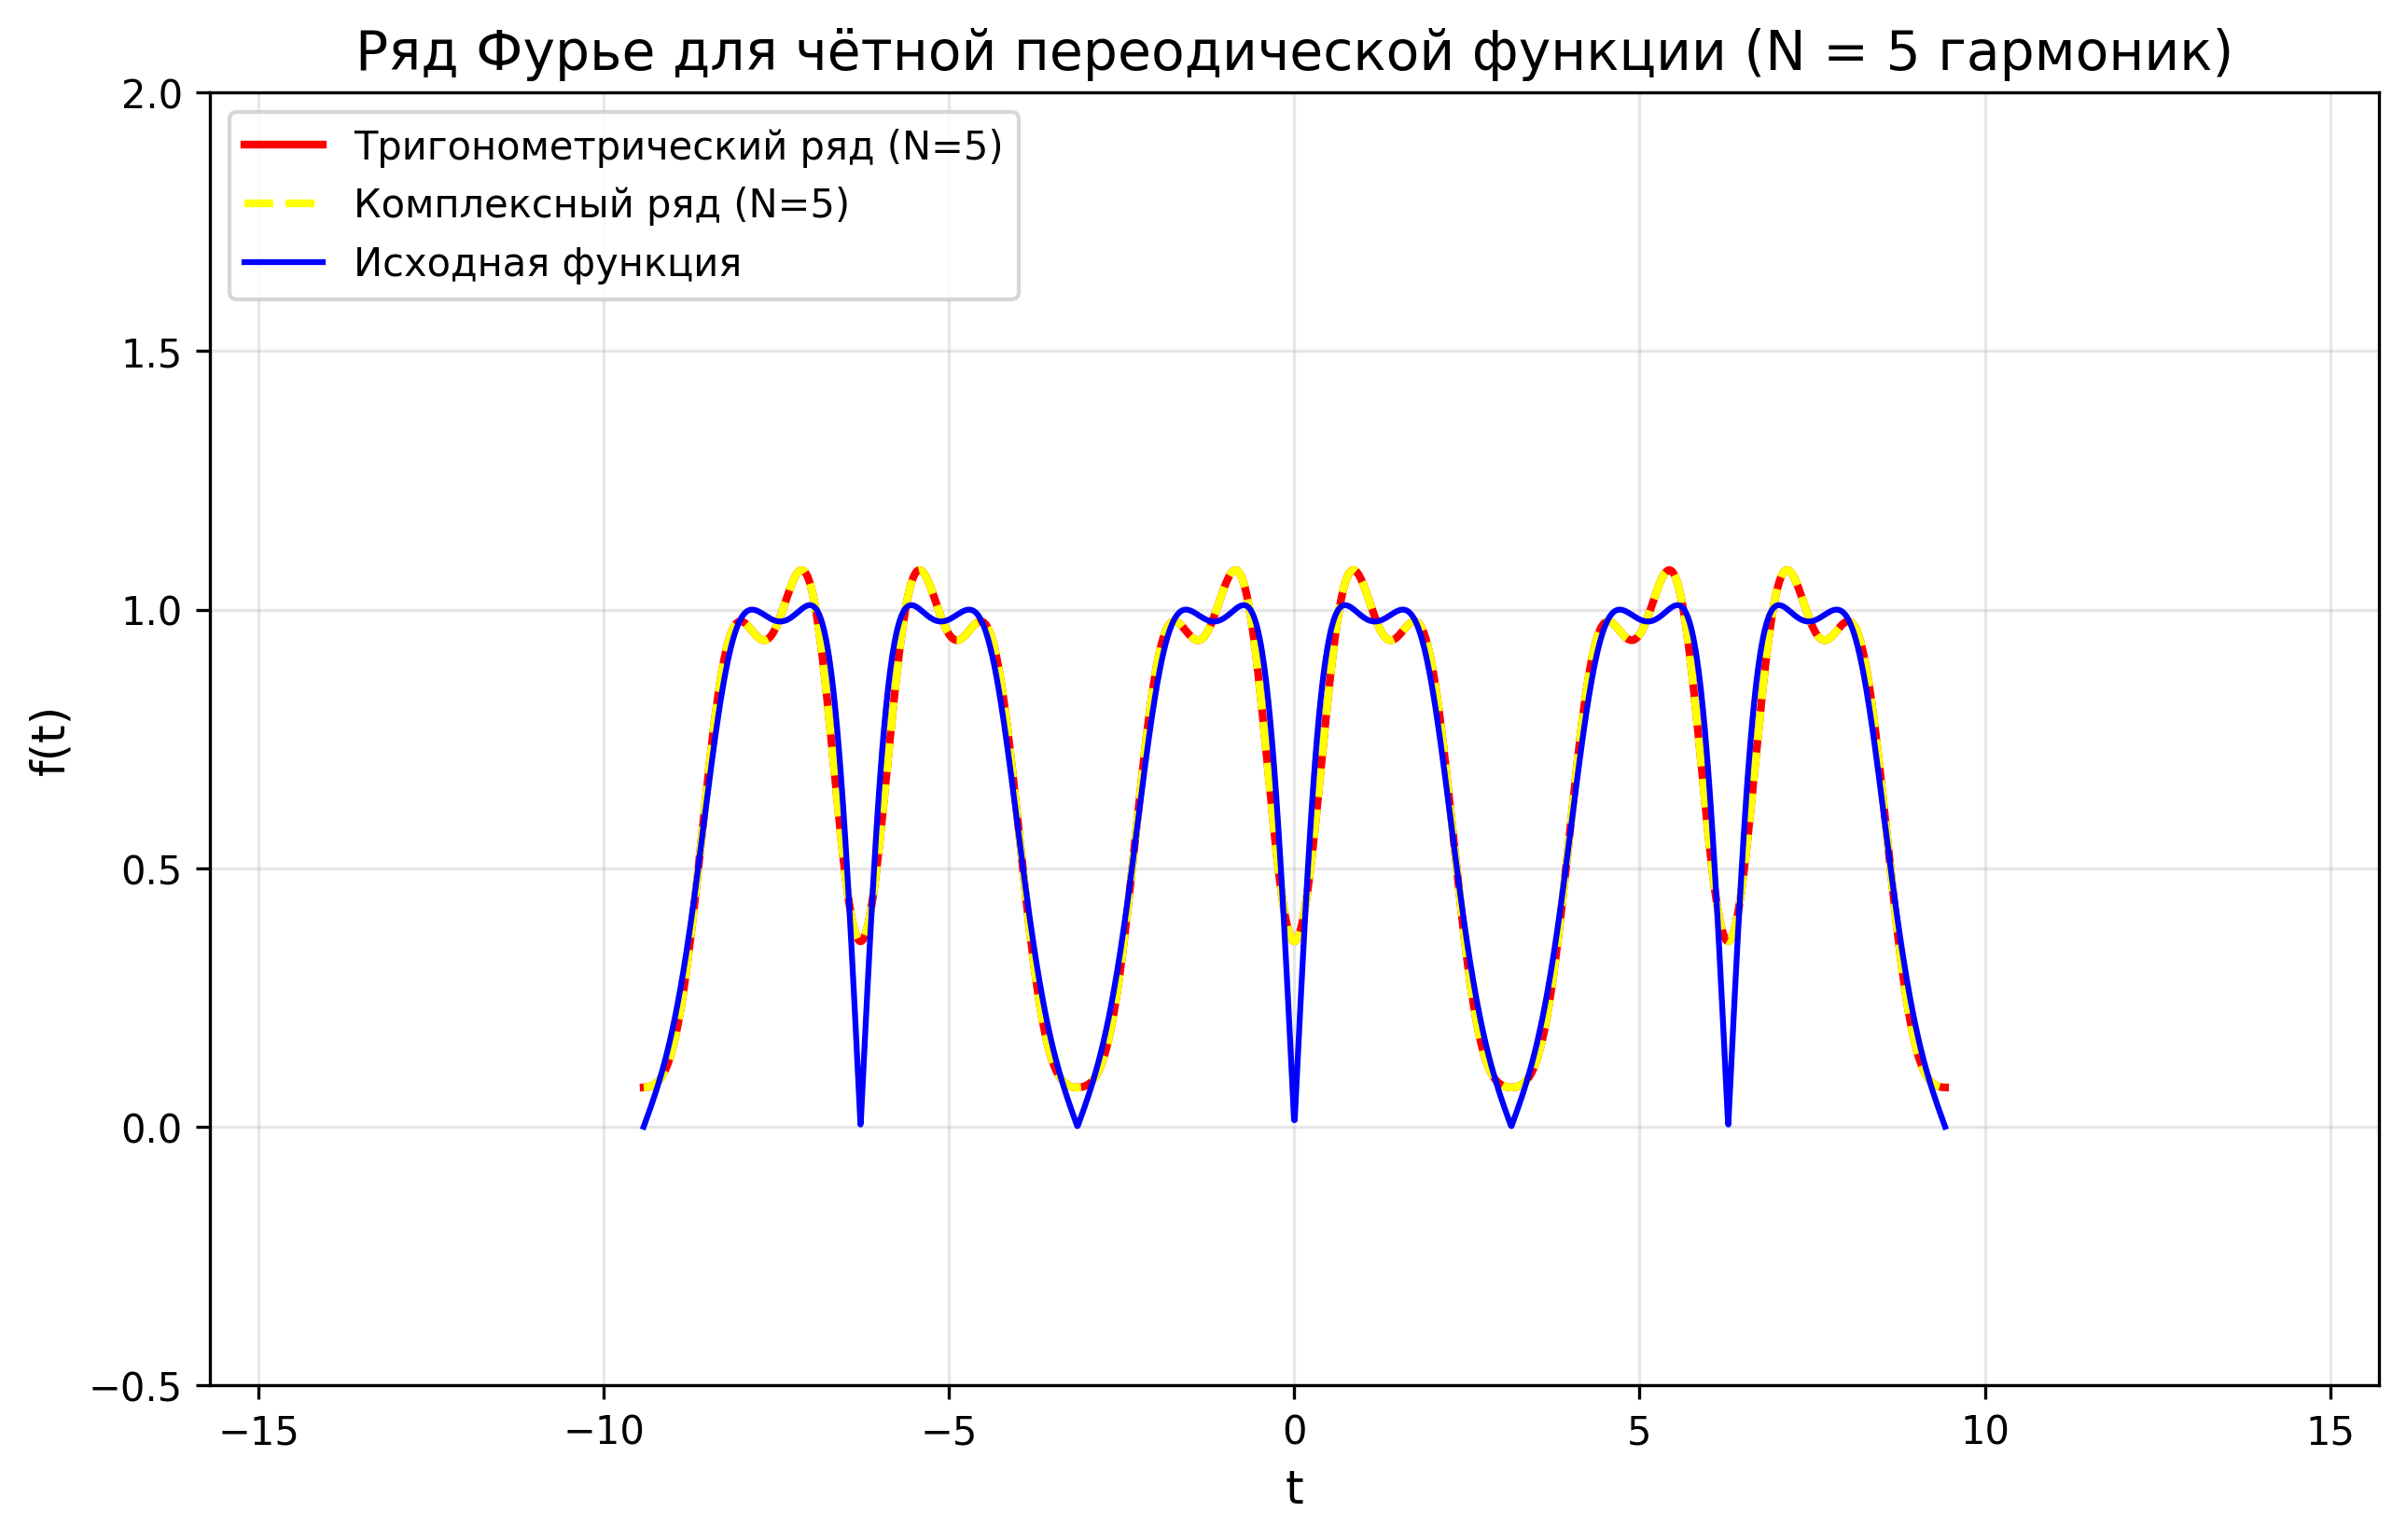
\includegraphics[width=\textwidth]{images/t2_5.png}
        \caption{N = 5 гармоник}
        \label{fig:n5}
    \end{subfigure}
    
    \vspace{0.5cm}
    
    \begin{subfigure}[b]{0.48\textwidth}
        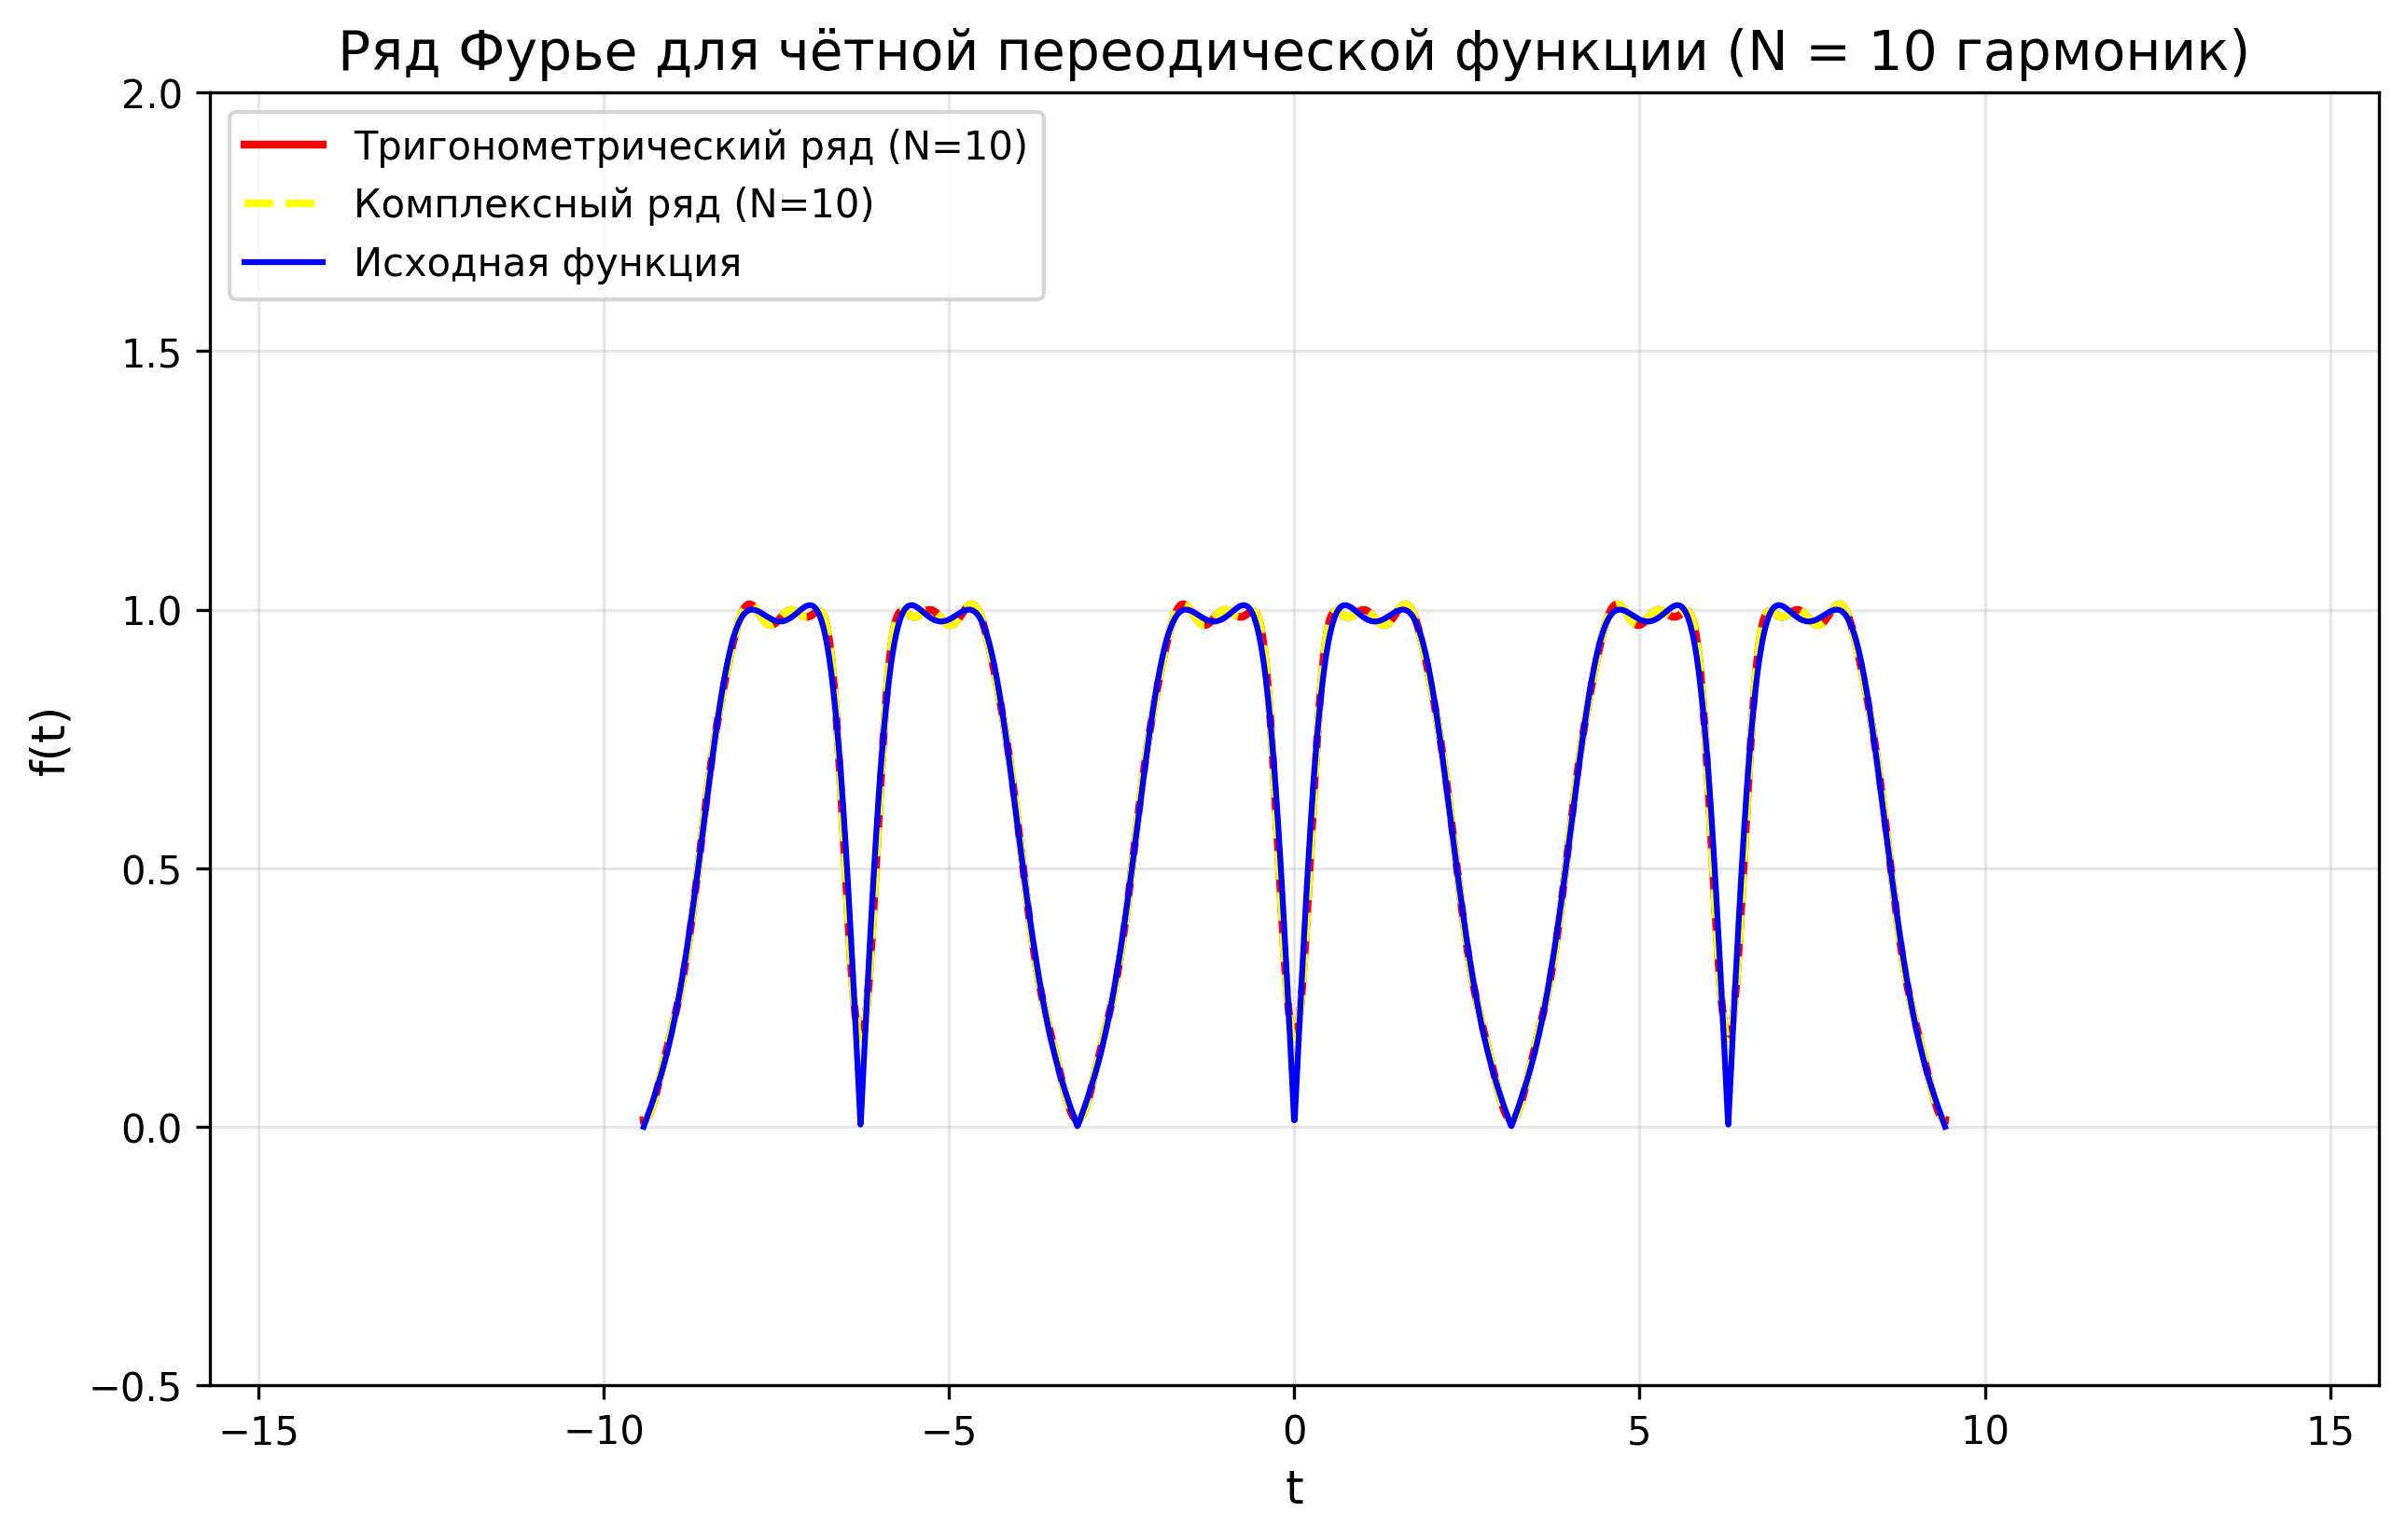
\includegraphics[width=\textwidth]{images/t2_10.png}
        \caption{N = 10 гармоник}
        \label{fig:n10}
    \end{subfigure}
    \hfill
    \begin{subfigure}[b]{0.48\textwidth}
        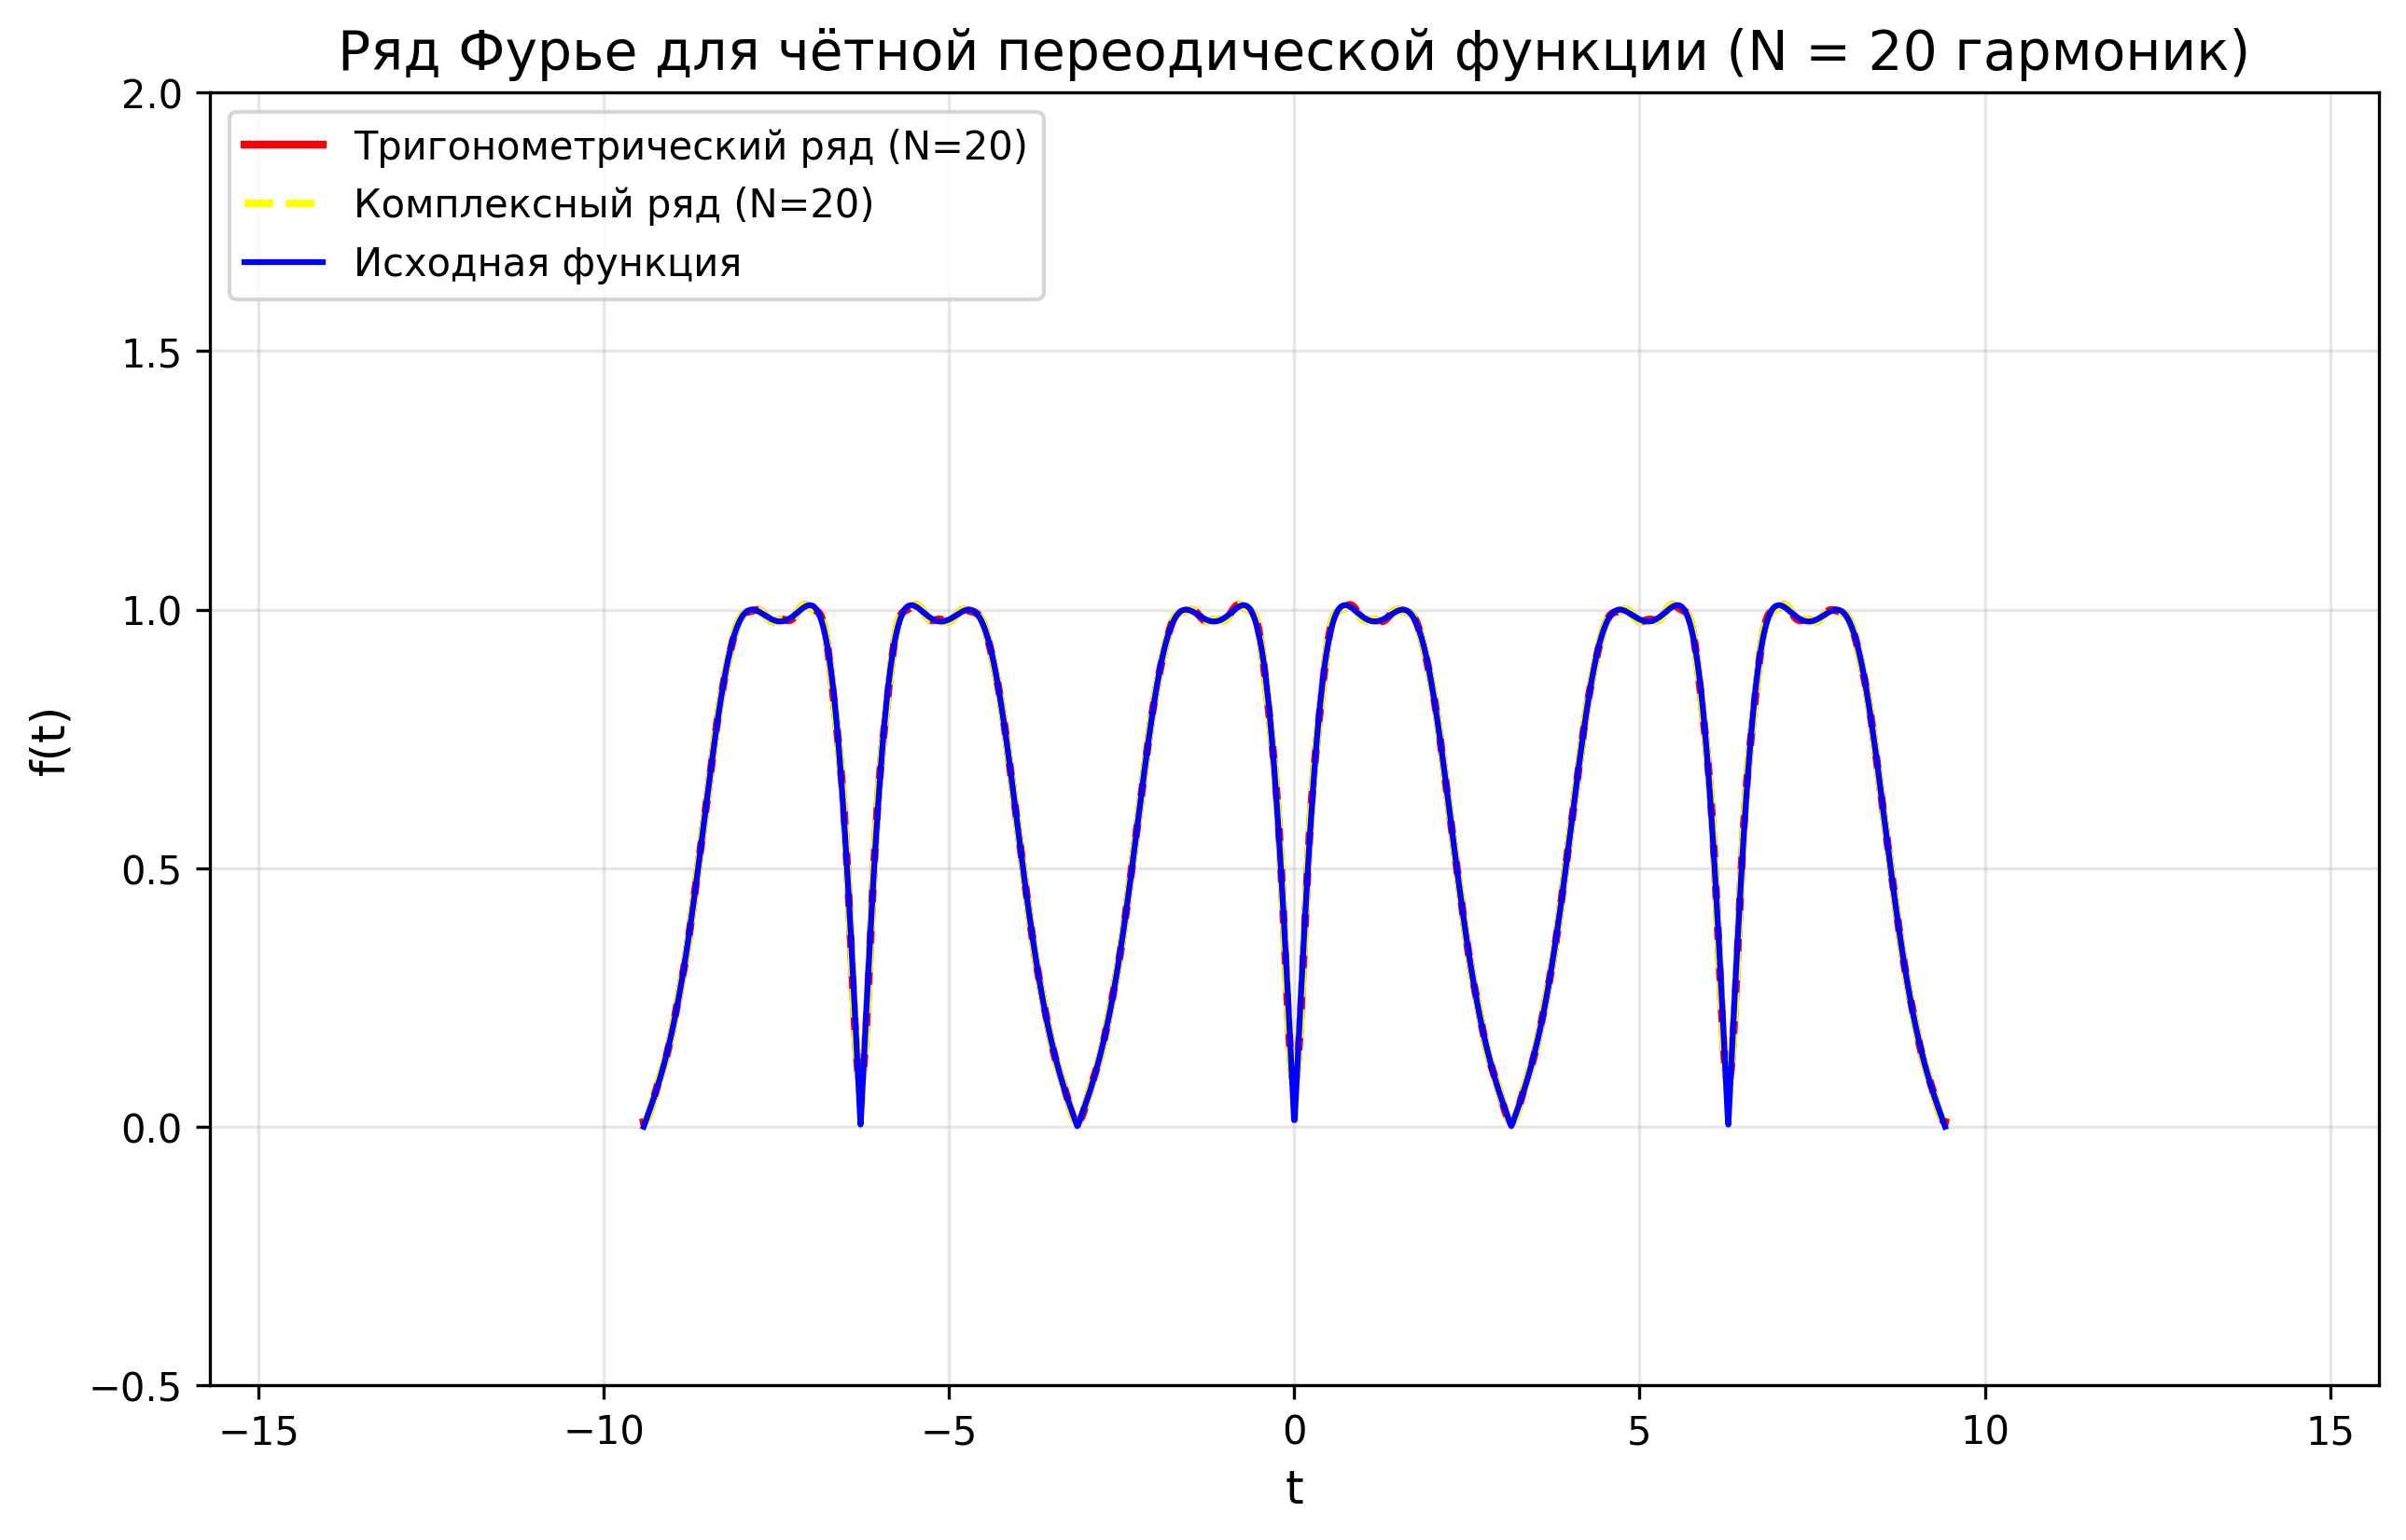
\includegraphics[width=\textwidth]{images/t2_20.png}
        \caption{N = 20 гармоник}
        \label{fig:n20}
    \end{subfigure}
    \vspace{0.5cm}
    \begin{subfigure}[b]{0.48\textwidth}
        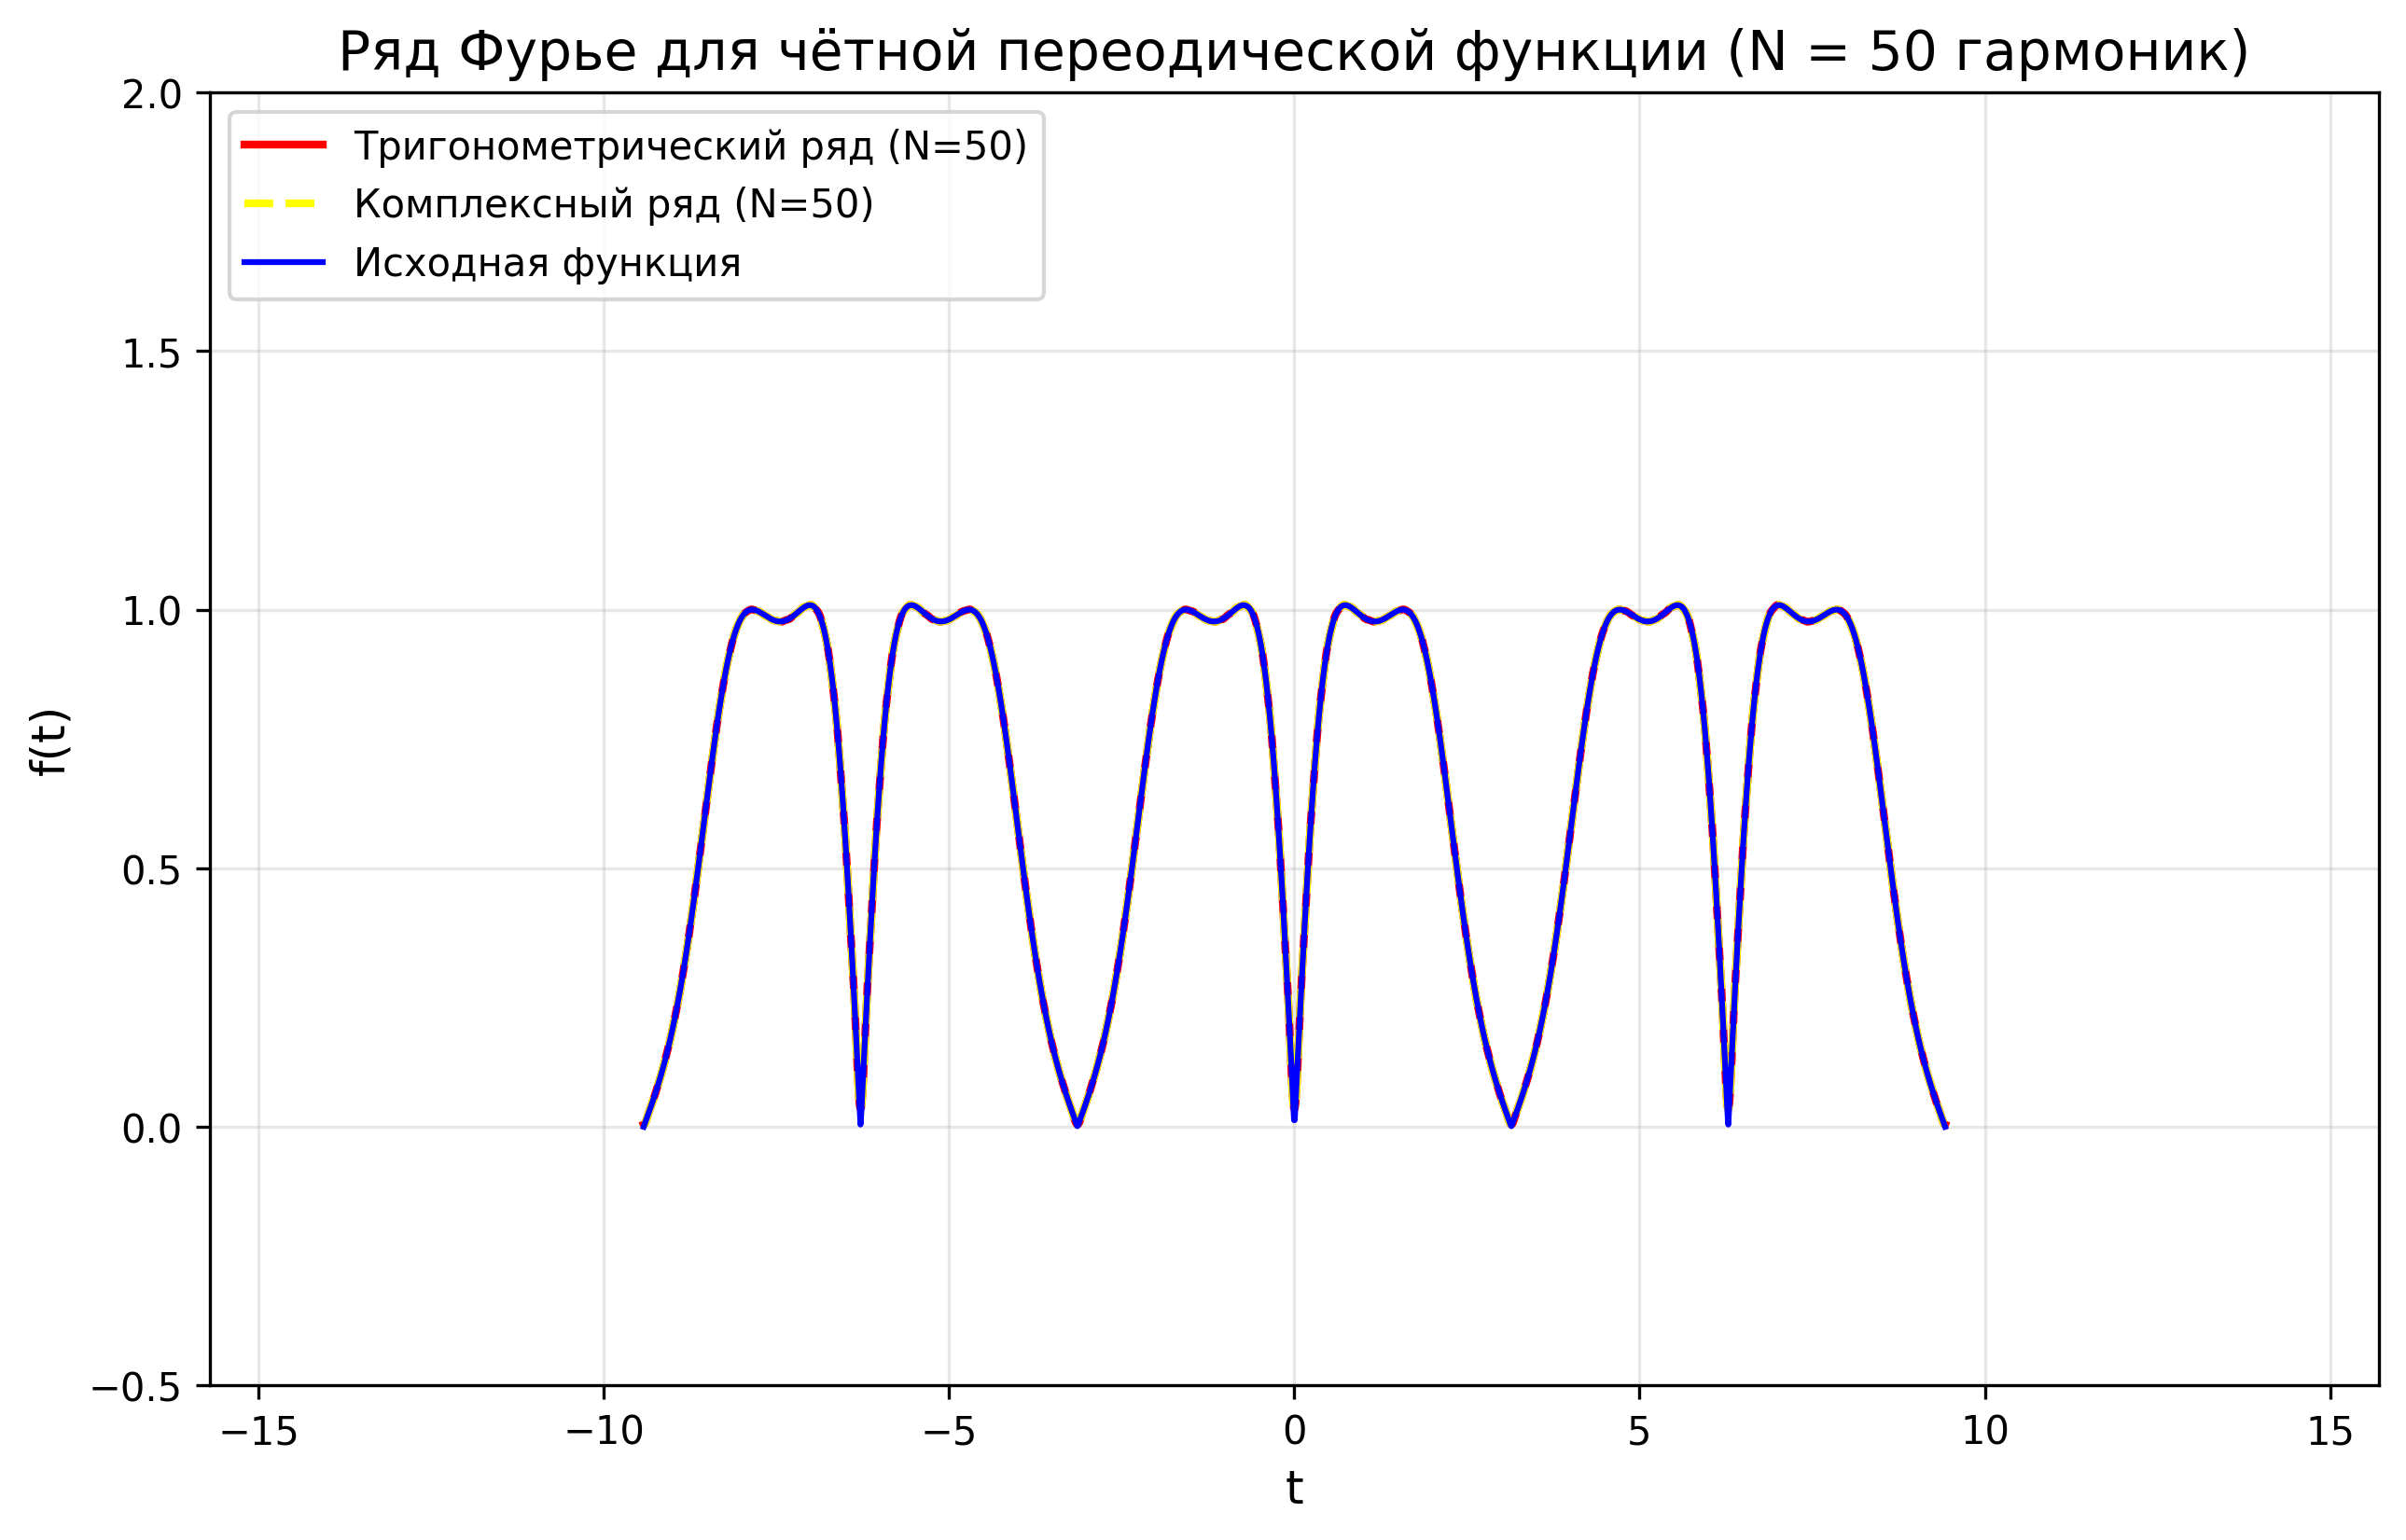
\includegraphics[width=\textwidth]{images/t2_50.png}
        \caption{N = 50 гармоник}
        \label{fig:n50}
    \end{subfigure}
        
    \caption{Приближение чётной переодической функции рядом Фурье для разного количества гармоник}
    \label{fig:fourier_grid}
\end{figure}


\newpage
\section{Приложение}
\begin{lstlisting}
    from matplotlib import pyplot as plt
import numpy as np
from numpy import pi, sin, cos, exp

t0 = 1
t1 = pi**2/5
t2 = pi*1.5

a = 2
b = 8

T = t2 - t0

def omega_n(n):
    return 2 * np.pi * n / T

def a_n(n):
    if n == 0:
        return (a * (t1 - t0) + b * (t2 - t1)) /T
    
    wn = omega_n(n)
    return (a * (sin(wn * t1) - sin(wn * t0)) + 
            b * (sin(wn * t2) - sin(wn * t1))) / (pi*n)

def b_n(n):
    wn = omega_n(n)
    return (a * (cos(wn * t0) - cos(wn * t1)) + 
            b * (cos(wn * t1) - cos(wn * t2))) / (pi*n)

def c_n(n):
    if n == 0:
        return (a * (t1 - t0) + b * (t2 - t1)) / T
    
    wn = omega_n(n)
    return (a * (exp(-1j * wn * t1) - exp(-1j * wn * t0)) + 
            b * (exp(-1j * wn * t2) - exp(-1j * wn * t1))) / (-1j * pi*n*2 )

def f(n):
    t = (n - t0) % T
    t = t0 + t
    
    if t0 <= t < t1:
        return a
    elif t1 <= t < t2:
        return b
    return 0

def F_n(n, x):
    res = 0
    n += 1

    for i in range(n):
        if i == 0:
            res += a_n(0)
        else:
            wn = omega_n(i)
            res += a_n(i)*cos(wn*x) + b_n(i)*sin(wn*x)
    return res

def G_n(n, x):
    res = 0
    for i in range((-n), n+1):
        wn = omega_n(i)
        res += c_n(i)*exp(1j*wn*x)
    return res.real



N_values = [1, 3, 5, 10, 20, 50] 
t = np.linspace(t0, t0 + 3*T, 1000)
x_original = np.array([f(val) for val in t])

for num in N_values:
    x_fur = F_n(num, t)
    x_fur2 = G_n(num, t)
    
    fig, ax = plt.subplots(figsize=(10, 6))
    
    ax.plot(t, x_fur, color="red", linewidth=2, label=f'Тригонометрический ряд (N={num})')
    ax.plot(t, x_fur2, color="yellow", linestyle='--', linewidth=2, label=f'Комплексный ряд (N={num})')
    ax.plot(t, x_original, color="blue", linewidth=1.5, label='Исходная функция')
    
    ax.set_xlabel('t', fontsize=12)
    ax.set_ylabel('f(t)', fontsize=12)
    ax.set_title(f'Ряд Фурье для квадратной волны (N = {num} гармоник)', fontsize=14)
    ax.set_xlim(t0- 2, t0 + 3*T+1)
    ax.set_ylim(0, 12)
    ax.legend(loc='upper left', fontsize=10)
    ax.grid(True, alpha=0.3)
    
    filename = f"t1_{num}.png"
    plt.savefig(filename, dpi=300, bbox_inches='tight')
    
    plt.show()
    plt.close(fig)
#for i in range(3):
 #   print(f"Коэффициент a_{i}: {a_n(i)}")
  #  print(f"Коэффициент b_{i}: {b_n(i)}")
   # print(f"Коэффициент c_{i}: {c_n(-i)}")


\end{lstlisting}

\end{document}
